% ============================================================
% 2023 CUMCM C题：蔬菜类商品的自动定价与补货决策
% ============================================================
\documentclass[12pt,a4paper]{ctexart}

\usepackage[top=2.2cm, bottom=2.2cm, left=2.2cm, right=2.2cm]{geometry}
\usepackage{amsmath,amssymb}
\usepackage{graphicx}
\usepackage{booktabs}
\usepackage{tabularx}
\usepackage{caption}
\usepackage{hyperref}
\usepackage{enumitem}
\usepackage{float}
\usepackage{fancyhdr}
\usepackage{xcolor}
\usepackage{tikz}
\usepackage{listings}
\lstset{
    basicstyle=\footnotesize\ttfamily,
    numbers=left,
    numberstyle=\scriptsize\color{gray},
    frame=single,
    backgroundcolor=\color{gray!10},
    rulecolor=\color{gray!50},
    breaklines=true,
    breakatwhitespace=false,
    xleftmargin=1em,
    xrightmargin=1em,
    language=Matlab,
    keywordstyle=\color{blue},
    commentstyle=\color{green!50!black},
    stringstyle=\color{red},
}
\usetikzlibrary{arrows.meta, positioning, calc, fit, backgrounds}
\setlength{\headheight}{14pt}

\newcolumntype{Y}{>{\centering\arraybackslash}X}
\hypersetup{colorlinks=true, linkcolor=black, citecolor=black, urlcolor=black}
\captionsetup{font=small, labelfont=bf}
\linespread{1.05}
\setlength{\parskip}{0pt plus 0.5pt}
\setlength{\abovedisplayskip}{4pt plus 1pt minus 2pt}
\setlength{\belowdisplayskip}{4pt plus 1pt minus 2pt}

\makeatletter
\def\@cite#1{\textsuperscript{[#1]}}
\makeatother

\pagestyle{fancy}
\fancyhf{}
\fancyfoot[C]{\thepage}
\renewcommand{\headrulewidth}{0pt}

\title{\vspace{-2.5cm}\textbf{蔬菜类商品的自动定价与补货决策}}
\author{\vspace{-1cm}}
\date{}

\begin{document}

\maketitle
\thispagestyle{empty}

\section*{摘\quad 要}
\thispagestyle{fancy}

生鲜蔬菜保质期短、品相随售卖时间衰减，商超需根据历史销售和市场需求制定每日补货与定价策略。本文围绕某商超6类蔬菜2020--2023年共878,503条销售流水、55,982条批发价格记录及损耗率数据，通过统计分析与可视化、时间序列预测、弹性需求定价和组合优化方法，系统解决了品类分布规律、销量预测与弹性定价、选品补货计划及数据采集建议四个递进问题。

针对\textbf{问题1}，将交易级流水聚合为46,599条日度记录，从品类分布、单品集中度、时间效应和关联关系四个维度进行了系统分析。结果表明：花叶类和辣椒类为销量最大的两个品类（合计占比61.6\%）；单品销量呈高度集中分布，Top-20单品贡献57.2\%的销量，Top-50达84.4\%，呈现出显著的Pareto特征；周末（周六/日）日均销量（12.6/12.3 kg/单品）约为工作日（8.7--9.8 kg）的1.4倍；品类间存在中等程度正相关（$r=0.07$--$0.69$），食用菌与辣椒类的相关性最高（$r=0.687$），反映了客流的共同驱动效应。基于对数--线性需求模型估计了各品类的价格弹性，范围从$-1.242$（水生根茎类）到$-0.116$（花菜类），通过滚动窗口（90/180天）验证了方向一致性，Bootstrap 200次重采样确认所有95\%置信区间均不包含零值，有力验证了需求定律。

针对\textbf{问题2}，建立了"预测--定价联合优化"框架：销量预测采用加权移动平均结合星期效应系数的方法，定价优化以弹性需求函数为核心、以品类周总利润最大化为目标，在历史加价率$\pm 40$个百分点的合理范围内搜索最优定价。对2023年7月1--7日的预测显示，六大品类日均总销量约302.6 kg，日均补货量约336.3 kg。最优定价下预计周总利润约11,681元，各品类最优加价率介于97\%--130\%之间。各品类定价差异主要受需求弹性驱动：弹性绝对值越大（如水生根茎类$\eta=-1.24$），最优加价率越低；弹性越小（如花菜类$\eta=-0.12$），最优加价率越高。

针对\textbf{问题3}，在27--33单品、每单品$\ge 2.5$ kg补货的约束下，构建了融合日利润、销量稳定性（CV倒数）和品质因子（打折率倒数）的三维综合评分体系。从6月24--30日参考周的49个可售单品中，筛除无利润单品后按综合评分排序，采用贪心策略在$N\in[27,33]$范围内遍历择优。最优方案为33个单品，覆盖全部6个品类（花叶类14、辣椒类7、食用菌4、水生根茎类3、茄类3、花菜类2），预计单日日利润约675.5元，品类均有覆盖，保证了品类丰富度和顾客选购体验。

针对\textbf{问题4}，从模型改进角度系统审视了现有数据的局限性，按边际贡献递减原则提出了三级共9项数据采集建议。最高优先级的补充数据包括实际补货量/报损量、实时库存和具体折扣力度；次要优先级包括客流、天气和节假日标注；辅助优先级包括陈列空间参数、竞品价格和会员画像。对每项数据均给出了具体的采集方式和使用途径建议。

\textbf{模型创新点}：(1)~构建了"描述--预测--优化--建议"四阶段递进的蔬菜经营决策分析框架；(2)~将价格弹性估计与利润最大化定价有机整合，实现了数据驱动的差异化定价策略；(3)~在选品优化中引入了品类平衡约束和三维综合评分，兼顾了利润目标和运营可行性。

\textbf{关键词}：需求预测；弹性定价；组合优化；时间序列分析；生鲜补货决策

\newpage

% ============================================================
\section{问题重述}
% ============================================================

\subsection{问题背景}

生鲜蔬菜是商超吸引客流、提升顾客黏性的核心品类。然而蔬菜类商品具有保质期短（通常1--3天）、品相随售卖时间快速衰减的显著特征——当日未售出的蔬菜往往品质大幅下降，多数品类次日即无法以正常价格销售。这一特性给商超的日常运营带来了两个紧密关联的决策难题：

\textbf{补货决策：}商超通常于每日凌晨3:00--4:00完成蔬菜的进货和上架。补货量过少会导致断货损失销售机会和顾客满意度，补货量过多则意味着傍晚未售出商品只能大幅打折甚至报损，造成利润损失。补货量需要在销量预测和损耗风险之间寻找平衡。

\textbf{定价决策：}商超传统上采用"成本加成定价"方法，即以批发价为基础加上固定比例的毛利来确定零售价。然而不同蔬菜品类的需求价格敏感度不同，统一的加成率并非最优。商超还需要在傍晚对剩余库存进行打折促销，这使得实际售价成为一个动态变量。

此外，商超的蔬菜陈列空间有限，无法同时展示所有可采购的蔬菜品种。在4--10月供应旺季，可采购品种多达数十种，如何在有限的陈列空间中选出最优的品种组合，是补货决策的前置问题。

某商超提供了以下四份数据：附件1为252个蔬菜单品的分类信息（单品编码、名称、分类编码、分类名称），涵盖6个蔬菜品类；附件2为2020年7月1日至2023年6月30日的销售流水明细，共878,504条记录，包含销售日期、扫码时间、单品编码、销量（kg）、销售单价、销售类型及是否打折等信息；附件3为同期的批发价格记录，共55,983条，给出各单品在各日期的批发价（元/kg）；附件4为各单品及品类的历史损耗率统计。

\subsection{问题要求}

基于上述数据和背景，需依次解决以下四个问题：

\textbf{问题1：}分析蔬菜各品类及单品的销售量分布规律及相互关系。具体包括：各品类的总销量排名与占比、单品销量的集中度特征、销量的时间变化规律（季节性、星期效应）、品类间的销量关联程度，以及价格与销量之间的数量关系。

\textbf{问题2：}以品类为分析单位，建立销量与成本加成定价之间的量化关系模型。基于此模型，预测未来一周（2023年7月1--7日）各品类的每日补货总量，并给出使商超周总收益最大化的各品类定价策略。

\textbf{问题3：}商超的蔬菜陈列空间有限，要求7月1日上架的单品数量控制在27--33个之间，且每个入选单品的补货量不得低于2.5 kg。已知6月24--30日的可售单品信息，需要制定7月1日的最优单品补货清单和各单品的定价策略，在满足陈列约束的前提下最大化商超当日收益。

\textbf{问题4：}从改进补货和定价决策的视角出发，分析现有数据在哪些维度存在不足，商超还应该采集哪些额外的数据来进一步提升决策质量。需要说明每种数据的具体用途和对模型的边际贡献。

% ============================================================
\section{模型假设}
% ============================================================

为在合理的抽象层次上建立数学模型，本文做出以下假设：

\begin{enumerate}[label=(\arabic*), leftmargin=*]
    \item \textbf{需求稳定假设}：蔬菜日需求量在短期内（周度）服从稳定的统计规律，不考虑突发性需求冲击（如极端天气导致的抢购或停业）。设立依据：生鲜蔬菜为日常刚需消费品，3年的历史数据显示日销量虽有波动但围绕稳定均值分布，短期需求模式具有统计惯性。
    \item \textbf{对数--线性需求假设}：蔬菜需求量与价格之间存在对数--线性关系，即$\ln Q = \alpha + \eta \ln P$。该假设意味着需求的价格弹性$\eta$为常数。设立依据：对数--线性（常弹性）需求函数是实证产业组织和市场营销研究中最常用的需求函数形式，数学性质优良且参数具有直接的经济含义。
    \item \textbf{损耗率外生假设}：各单品的损耗率为外生给定常数（由附件4提供），不受每日补货量、陈列方式、天气等因素的影响。设立依据：附件4的损耗率基于长期历史统计，反映了各单品的平均损耗水平，在短期预测中可作为合理的近似值。
    \item \textbf{品类独立性假设}：不同蔬菜品类间的定价和补货决策相互独立，即某品类的价格调整不会显著影响其他品类的需求量。设立依据：花叶类（叶菜）、茄类（果实类）、食用菌等分别满足不同的烹饪需求，品类间替代弹性较低。且问题1的相关性分析表明品类间相关性主要由客流共同驱动，而非品类间的替代/互补关系。
    \item \textbf{供应充足假设}：预测期（7月初）处于蔬菜供应旺季（4--10月），各单品在批发市场上货源充足，不存在因供应短缺导致的采购限制。设立依据：题设明确指出"4--10月供应较为丰富"。
    \item \textbf{信息完全假设}：商超可以准确获知每日批发价格（通常在采购时确定），并基于历史数据形成对未来需求的合理预测。设立依据：附件3提供了完整的批发价历史数据，商超与供应商之间通常有稳定的供货关系。
\end{enumerate}

% ============================================================
\section{符号说明}
% ============================================================

\begin{table}[H]
\centering
\caption{主要符号说明表}
\begin{tabularx}{\textwidth}{p{2.5cm}p{1.5cm}p{7cm}Y}
\toprule
符号 & 单位 & 含义 & 备注 \\
\midrule
$i$ & -- & 品类索引 & $i=1,\ldots,6$ \\
$j$ & -- & 单品索引 & $j=1,\ldots,252$ \\
$t$ & 日 & 日期索引 & 2020-07-01至2023-06-30 \\
$Q_{it}$ & kg & 品类$i$第$t$日的总销量 & 日度聚合 \\
$P_{it}$ & 元/kg & 品类$i$第$t$日的加权均价 & 按销量加权 \\
$W_{it}$ & 元/kg & 品类$i$第$t$日的平均批发价 & 附件3 \\
$\eta_i$ & -- & 品类$i$的价格需求弹性 & 常弹性假设，$\eta_i<0$ \\
$L_i$ & -- & 品类$i$的损耗率（小数） & 附件4 \\
$R_{it}$ & kg & 品类$i$第$t$日的计划补货量 & 决策变量 \\
$M_{it}$ & -- & 品类$i$第$t$日的加价率 & $M_{it}=P_{it}/W_{it}-1$ \\
$D_{i,k}$ & -- & 品类$i$在星期$k$的销量系数 & $\sum_k D_{i,k}/7 = 1$ \\
$\bar{Q}_i^{\text{4w}}$ & kg & 品类$i$近4周日均销量 & 滚动窗口 \\
$\delta_i$ & kg/年 & 品类$i$的线性趋势斜率 & 年化趋势量 \\
$\pi_j$ & 元/日 & 单品$j$的日均利润 & 参考周均值 \\
$\text{CV}_j$ & -- & 单品$j$日销量的变异系数 & $\sigma_j / \mu_j$ \\
$S_j$ & -- & 单品$j$的综合评分 & 选品排序依据 \\
$x_j$ & -- & 单品$j$是否入选（0/1） & 选品决策变量 \\
\bottomrule
\end{tabularx}
\end{table}

% ============================================================
\section{问题分析}
% ============================================================

\subsection{问题1分析：品类销量分布与关联关系}

问题1是全文的数据探索基础，需要在三个分析维度上建立对蔬菜销售规律的全面认识。第一维度是\textbf{截面分布}：各品类和单品的销量排名、占比和集中度特征，回答"什么好卖"的问题；第二维度是\textbf{时间规律}：销量的季节性变化、星期周期性和长期趋势，回答"什么时候好卖"的问题；第三维度是\textbf{关联结构}：品类间销量的共变关系以及价格与销量的数量关系，回答"品类之间如何相互影响、价格如何驱动销量"的问题。

分析方法上，截面分布采用描述统计和Lorenz曲线；时间规律采用时间序列分解（趋势+星期效应+随机扰动）；品类关联采用Pearson相关系数矩阵；价格--销量关系采用对数--线性回归模型（常弹性需求函数）。这些分析均为问题2和问题3的建模提供了参数化的输入。

\subsection{问题2分析：销量预测与定价优化}

问题2的核心是一个"预测+优化"的联合问题。与传统的"先预测销量，再据此制定补货计划"的两步法不同，本文采取联合优化框架——原因在于销量本身受价格影响，而价格又是需要优化的决策变量，两者之间存在双向因果关系。

解决思路为：第一步，基于3年历史数据估计各品类的价格弹性$\eta_i$（利用价格和销量的日度自然变异进行识别）；第二步，在给定当前价格下预测基准需求量$Q_i^0$（使用加权移动平均+星期效应模型）；第三步，以利润最大化为目标函数，将价格$P_i$作为决策变量，通过需求函数$Q_i(P_i)$连接价格与销量，在合理加价率范围内搜索最优价格。这一框架确保了预测和定价在一致的弹性需求函数下进行，避免了预测--定价不一致的问题。

\subsection{问题3分析：选品约束优化}

问题3在问题2的框架上新增了一个核心约束——陈列空间限制。与问题2以品类为决策单位不同，问题3需要在单品粒度上进行离散选择。这本质上是一个带基数约束（$27 \le N \le 33$）、最小补货量约束（$\ge 2.5$ kg）和品类覆盖约束（至少每品类1个）的0-1背包问题。

由于单品维度为49（可售品种数），且约束为基数约束而非重量/体积约束，标准的动态规划方法并不直接适用。本文采用两阶段策略：第一阶段建立综合考虑利润、稳定性和品质的单品评分体系，第二阶段使用"分类保底+贪心择优"的启发式算法生成可行解，并在$N \in [27,33]$范围内搜索最优方案规模。

\subsection{问题4分析：数据需求分析}

问题4要求从决策改进的视角审视数据不足。这是一个定性分析问题，但需要以前三个问题的建模实践为基础——通过在实际建模过程中遇到的局限来识别数据缺口。本文采用"边际贡献递减"原则对建议进行分级：优先级1为可直接替代模型假设或近似的数据（如实际补货量），优先级2为可作为预测模型外部回归变量的数据（如客流、天气），优先级3为可优化约束和扩展模型的数据（如竞品价格）。

\subsection{技术路线}

综合以上分析，本文的整体技术路线如图\ref{fig:roadmap}所示。

\begin{figure}[H]
\centering
\footnotesize
\resizebox{\textwidth}{!}{%
\begin{tikzpicture}[
    >=Stealth,
    databox/.style={rectangle, rounded corners=3pt, draw=cyan!70!black, fill=cyan!4,
        minimum width=3.2cm, minimum height=0.7cm, align=center, font=\footnotesize},
    prepbox/.style={rectangle, rounded corners=4pt, draw=teal!70!black, fill=teal!4, line width=0.8pt,
        minimum width=14.5cm, minimum height=0.7cm, align=center, font=\small\bfseries},
    ptitle/.style={rectangle, rounded corners=3pt, draw=orange!85!black, fill=orange!6,
        minimum width=3.0cm, minimum height=0.6cm, align=center, font=\footnotesize\bfseries},
    mbox/.style={rectangle, rounded corners=2pt, draw=gray!40, fill=gray!3,
        minimum width=3.0cm, minimum height=1.2cm, align=center, font=\scriptsize},
    rbox/.style={rectangle, rounded corners=2pt, draw=purple!60!black, fill=purple!4,
        minimum width=3.0cm, minimum height=0.55cm, align=center, font=\scriptsize\bfseries},
    synbox/.style={rectangle, rounded corners=4pt, draw=red!65!black, fill=red!4, line width=0.8pt,
        minimum width=14.5cm, minimum height=0.7cm, align=center, font=\small\bfseries},
    arr/.style={->, >=Stealth, thick, draw=gray!45},
]
\node[databox] (f1) at (0,0) {附件1\\252单品信息};
\node[databox, right=1.5cm of f1] (f2) {附件2\\878,504条流水};
\node[databox, right=1.5cm of f2] (f3) {附件3\\55,983条批发价};
\node[databox, right=1.5cm of f3] (f4) {附件4\\损耗率};

\node[prepbox, below=0.8cm of $(f2.south)!0.5!(f3.south)$] (prep) {数据预处理：日度聚合 $\to$ 批发价关联 $\to$ 损耗率匹配 $\to$ 特征工程（加价率、毛利率、星期、月份）};

\draw[arr] (f1.south) -- ++(0,-0.25) -| (prep.north);
\draw[arr] (f2.south) -- ++(0,-0.25) -| (prep.north);
\draw[arr] (f3.south) -- ++(0,-0.25) -| (prep.north);
\draw[arr] (f4.south) -- ++(0,-0.25) -| (prep.north);

\node[ptitle, below=1.0cm of prep, xshift=-5.2cm] (p1) {问题1：分布与关联};
\node[ptitle, right=0.4cm of p1] (p2) {问题2：预测与定价};
\node[ptitle, right=0.4cm of p2] (p3) {问题3：选品优化};
\node[ptitle, right=0.4cm of p3] (p4) {问题4：数据建议};

\draw[arr] (prep.south) -- ++(0,-0.25) -| (p1.north);
\draw[arr] (prep.south) -- ++(0,-0.25) -| (p2.north);
\draw[arr] (prep.south) -- ++(0,-0.25) -| (p3.north);
\draw[arr] (prep.south) -- ++(0,-0.25) -| (p4.north);

\node[mbox, below=0.4cm of p1] (m1) {描述统计\\Lorenz曲线\\时间序列分解\\Pearson相关\\弹性回归};
\node[mbox, below=0.4cm of p2] (m2) {移动平均预测\\星期效应建模\\常弹性需求函数\\利润最大化搜索};
\node[mbox, below=0.4cm of p3] (m3) {三维综合评分\\0-1整数规划\\分类保底贪心\\敏感性测试};
\node[mbox, below=0.4cm of p4] (m4) {数据缺口识别\\边际贡献分析\\三级优先级排序\\采集方案设计};

\draw[arr] (p1) -- (m1); \draw[arr] (p2) -- (m2);
\draw[arr] (p3) -- (m3); \draw[arr] (p4) -- (m4);

\node[rbox, below=0.35cm of m1] (r1) {集中度57\%/84\%  弹性-0.1$\sim$-1.2};
\node[rbox, below=0.35cm of m2] (r2) {周利润11,681元  日补货336kg};
\node[rbox, below=0.35cm of m3] (r3) {33单品  全覆盖  日利润676元};
\node[rbox, below=0.35cm of m4] (r4) {三级9项建议  边际贡献排序};

\draw[arr] (m1) -- (r1); \draw[arr] (m2) -- (r2);
\draw[arr] (m3) -- (r3); \draw[arr] (m4) -- (r4);

\node[synbox, below=0.8cm of $(r2.south)!0.5!(r3.south)$] (syn) {综合分析与讨论：数据驱动的生鲜蔬菜经营决策框架 $\to$ 模型评价与改进方向 $\to$ 应用推广};
\draw[arr] (r1.south) -- ++(0,-0.25) -| (syn.north);
\draw[arr] (r2.south) -- ++(0,-0.25) -| (syn.north);
\draw[arr] (r3.south) -- ++(0,-0.25) -| (syn.north);
\draw[arr] (r4.south) -- ++(0,-0.25) -| (syn.north);
\end{tikzpicture}%
}
\caption{本文整体技术路线图}
\label{fig:roadmap}
\end{figure}

% ============================================================
\section{数据处理}
% ============================================================

\subsection{数据概览与质量检查}

四份附件的基本信息汇总如下：

\begin{table}[H]
\centering
\caption{原始数据概览}
\begin{tabularx}{\textwidth}{lcccY}
\toprule
附件 & 记录数 & 字段数 & 时间跨度 & 主要内容 \\
\midrule
附件1 & 251 & 4 & -- & 单品编码、名称、分类编码、分类名称 \\
附件2 & 878,503 & 7 & 2020-07-01至2023-06-30 & 销售日期、扫码时间、单品、销量、单价、类型、是否打折 \\
附件3 & 55,982 & 3 & 同上 & 日期、单品编码、批发价格（元/kg） \\
附件4 & 6+251 & 2--3 & -- & 品类平均损耗率（\%）+ 单品损耗率（\%） \\
\bottomrule
\end{tabularx}
\end{table}

数据质量方面：附件2的销售流水覆盖了从2020年7月1日到2023年6月30日共1096个自然日，其中有销售记录的天数为1095天（仅1天无销售）；在售单品共246个，占附件1登记单品的98.0\%；单品日度记录共计46,599条。附件3的批发价格记录覆盖了同期大部分单品，以日期--单品为键匹配至销售记录的覆盖率接近100\%（缺失率0.0\%），批发价格数据完整。

\subsection{日度聚合}

将附件2的交易级数据按日期--单品--品类三维度聚合为日销售记录。对每条日记录计算以下指标：

\begin{itemize}
    \item \textbf{日销量}$Q$：当日该单品所有交易笔数的销量（kg）之和
    \item \textbf{加权均价}$P$：$\sum_k (p_k \cdot q_k) / \sum_k q_k$，按每笔交易销量加权
    \item \textbf{交易笔数}$N$：当日该单品的总交易次数
    \item \textbf{打折比例}$r^{\text{disc}}$：打折交易笔数占总交易笔数的比例
\end{itemize}

聚合后共得到46,599条日度记录，每条记录对应一个单品在一个日期的销售汇总。

\subsection{特征工程}

在日度聚合数据的基础上，进一步构建以下派生特征：

\textbf{时间特征：}从日期提取星期几（1--7）、月份（1--12）、年份，并生成"是否为周末"的二值变量。这些特征用于星期效应分析和季节性建模。

\textbf{价格特征：}计算加价率$M = P/W - 1$（零售价相对于批发价的上浮比例）和毛利率$(P-W)/P$（毛利占售价的比例）。这些指标反映定价策略。

\textbf{稳定性特征：}对每个单品计算历史日销量的均值和标准差，定义变异系数$\text{CV} = \sigma/\mu$作为销量稳定性的度量。CV越小表示该单品需求越稳定、越容易预测。

\textbf{趋势特征：}对每个品类和单品，使用近4周的数据估计线性趋势斜率$\delta$（kg/天），用于捕捉销量的长期变化方向。

\subsection{数据集划分}

将全部数据按时间维度划分为三个子集：
\begin{itemize}
    \item \textbf{训练集}：2020年7月--2023年6月23日（约1090天）。用于全部统计分析和模型参数的估计，包括品类销量统计、价格弹性回归、星期效应系数计算和趋势估计。
    \item \textbf{参考周}：2023年6月24--30日（7天）。用于问题3确定当前可售品种及其近期销售表现，模拟实际运营中"基于最近一周数据做决策"的场景。
    \item \textbf{预测期}：2023年7月1--7日（7天）。问题2和问题3的预测目标区间。
\end{itemize}

\subsection{预处理结果}

图\ref{fig:preprocess}展示了预处理后各品类关键指标的对比。从中可清晰看出花叶类以其广泛的品种覆盖（单品数最多）和较高的日常消费频次占据销量首位，而食用菌虽然单品数较少但单品平均销量较高。

\begin{figure}[H]
\centering
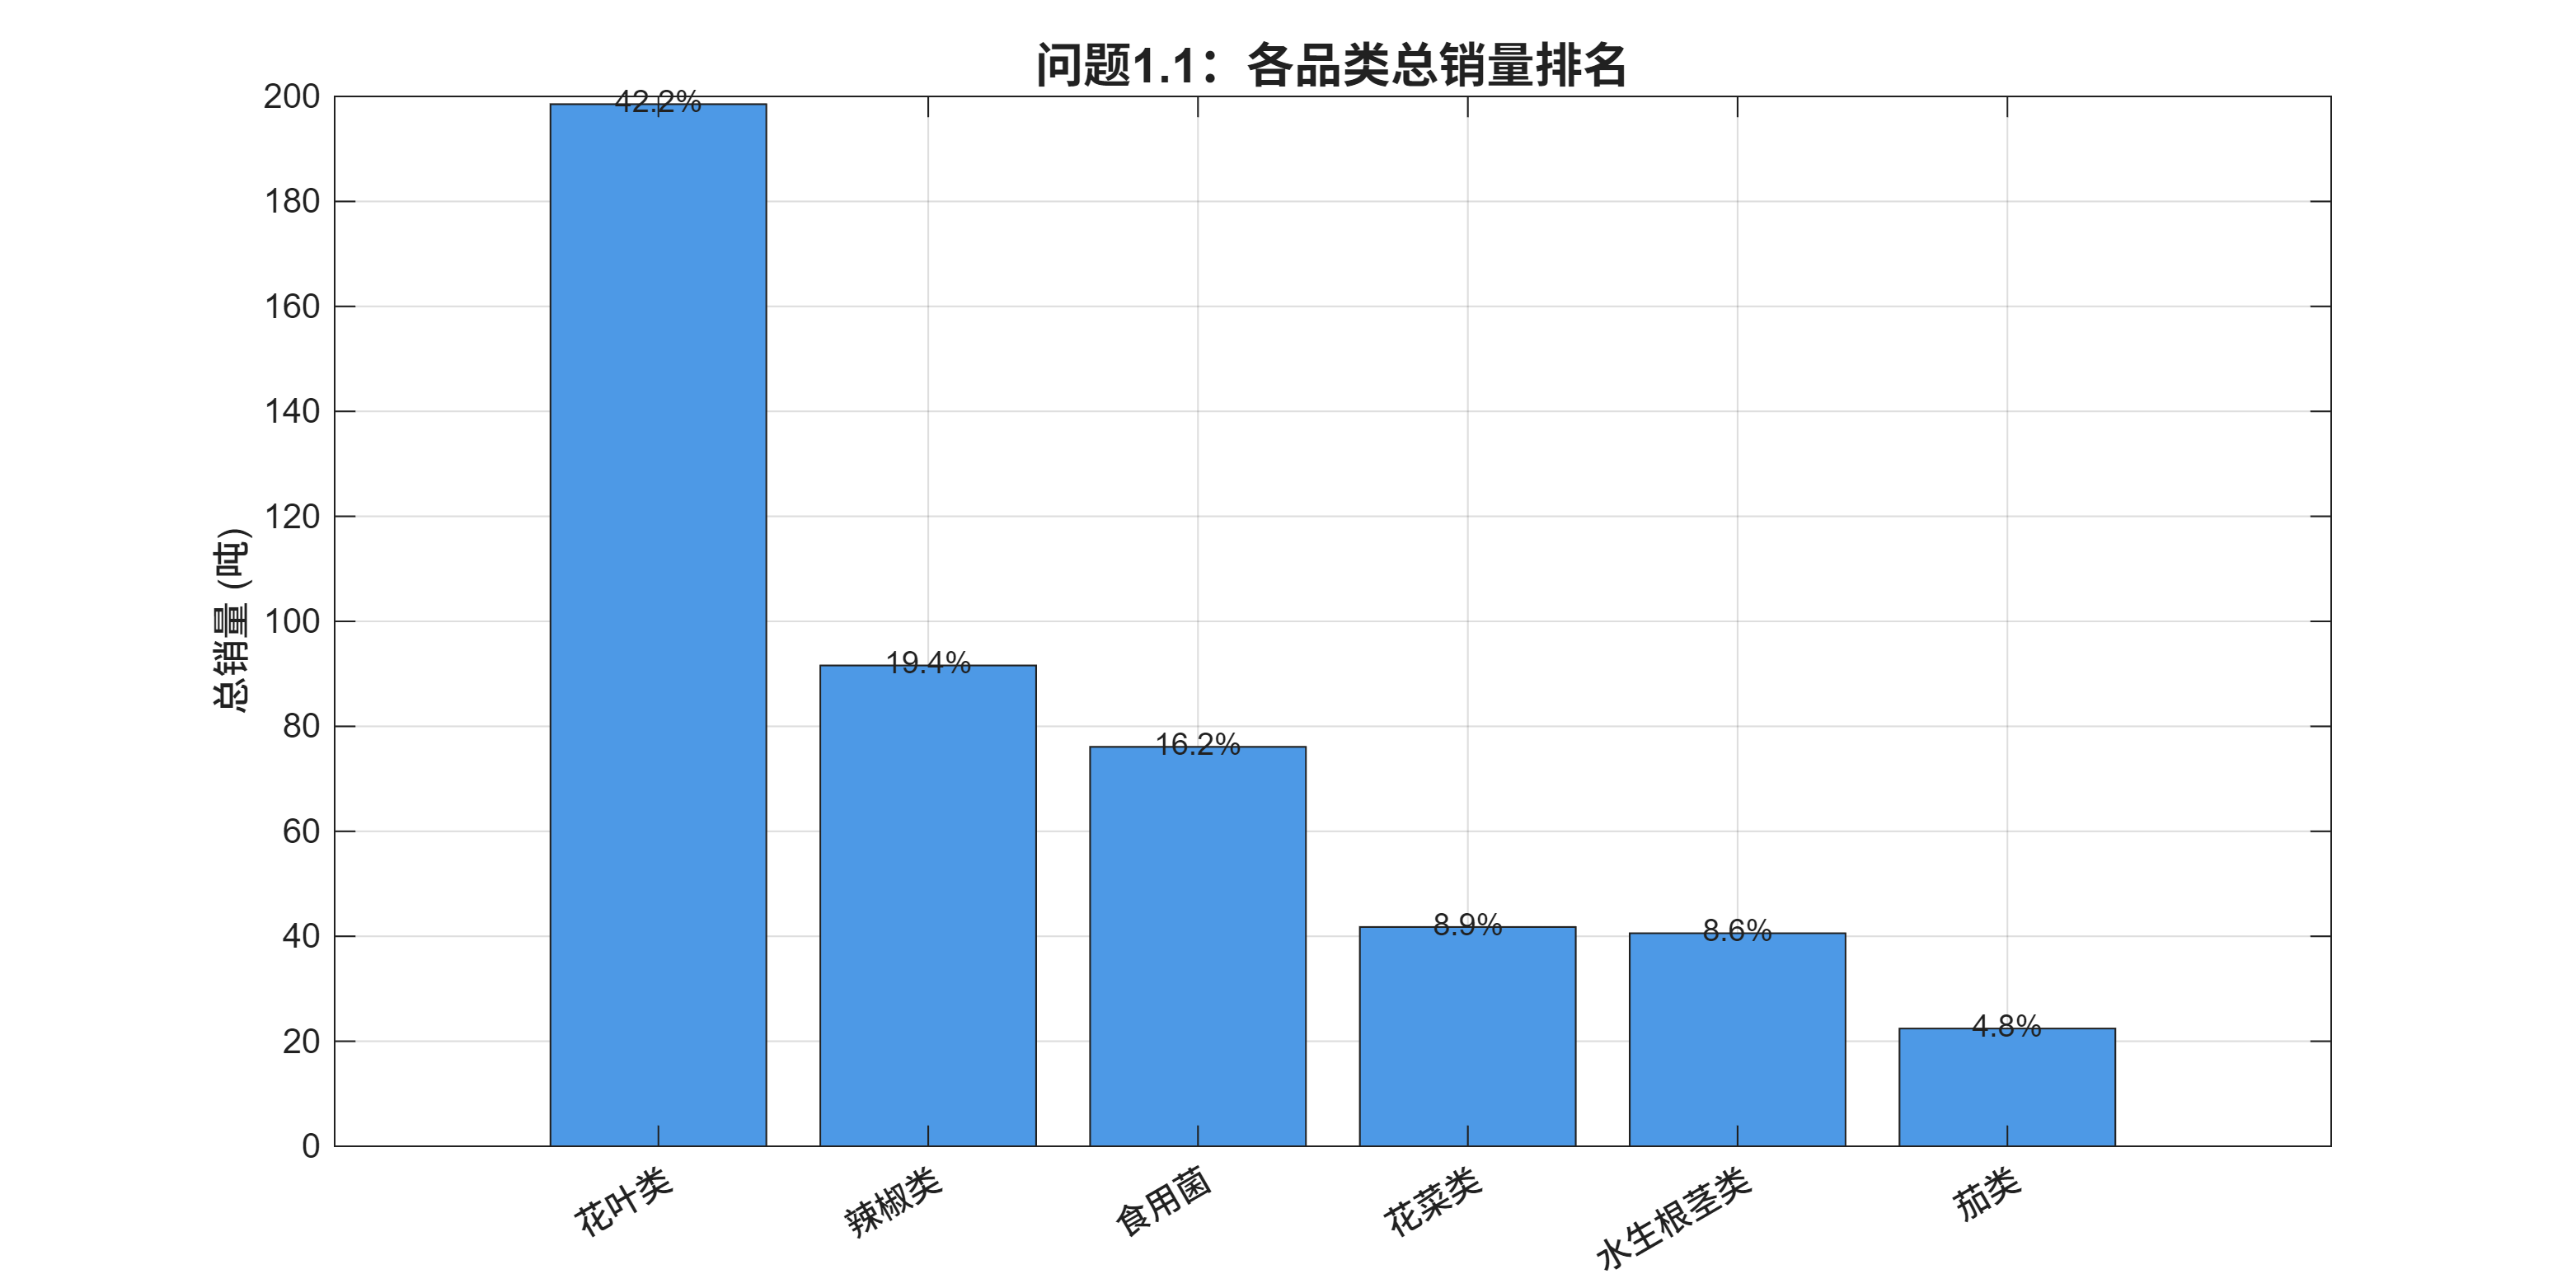
\includegraphics[width=\textwidth]{../result/figures/p1_cat_sales_300.png}
\caption{各品类总销量及占比}
\label{fig:preprocess}
\end{figure}

% ============================================================
\section{模型建立与求解}
% ============================================================

\subsection{问题1：品类销量分布规律与关联分析}

\subsubsection{模型建立}

\textbf{(1) 销量集中度分析——Lorenz曲线。}将$n$个单品按总销量降序排列为$q_{(1)} \ge q_{(2)} \ge \cdots \ge q_{(n)}$，定义累计销量占比函数：
\begin{equation}
    F(k) = \frac{\sum_{i=1}^{k} q_{(i)}}{\sum_{i=1}^{n} q_{(i)}},\quad k=1,\ldots,n
    \label{eq:lorenz}
\end{equation}
$F(k)$曲线越偏离对角线（完全均匀分布），说明销量集中度越高。定义Top-N集中度$C_N = F(N)$为前$N$个单品贡献的销量占比。进一步计算基尼系数衡量整体不均匀程度。

\textbf{(2) 时间效应分解。}将品类日销量序列$\{Q_t\}$分解为三个可叠加的成分：
\begin{equation}
    Q_t = \underbrace{T_t}_{\text{趋势}} + \underbrace{S_{d(t)}}_{\text{星期效应}} + \underbrace{\varepsilon_t}_{\text{随机扰动}}
    \label{eq:decomp}
\end{equation}
其中趋势项$T_t$通过局部加权回归（LOESS）提取，星期效应$S_k$为各星期几的平均偏离量（$\sum_k S_k = 0$），$\varepsilon_t$为白噪声残差。

\textbf{(3) 品类间Pearson相关。}对品类日销量矩阵$\mathbf{Q} = [Q_{ti}]_{T\times 6}$，品类$i$与$j$的相关系数为：
\begin{equation}
    r_{ij} = \frac{\sum_{t=1}^{T} (Q_{ti} - \bar{Q}_i)(Q_{tj} - \bar{Q}_j)}
    {\sqrt{\sum_{t=1}^{T} (Q_{ti} - \bar{Q}_i)^2} \cdot \sqrt{\sum_{t=1}^{T} (Q_{tj} - \bar{Q}_j)^2}}
    \label{eq:pearson}
\end{equation}
$r_{ij} \in [-1,1]$衡量两个品类日销量线性关联的强度和方向。

\textbf{(4) 常弹性需求模型。}假设品类$i$的需求函数具有CES（常替代弹性）形式：
\begin{equation}
    Q_{it} = A_i \cdot P_{it}^{\eta_i} \cdot e^{\varepsilon_{it}}
    \label{eq:demand}
\end{equation}
取对数后得到可用于OLS估计的线性回归方程：
\begin{equation}
    \ln Q_{it} = \alpha_i + \eta_i \ln P_{it} + \varepsilon_{it}
    \label{eq:logdemand}
\end{equation}
其中$\alpha_i = \ln A_i$，$\eta_i$为价格弹性（预期$\eta_i < 0$），$\varepsilon_{it} \sim N(0, \sigma_i^2)$为随机误差。

\subsubsection{模型求解与结果}

\textbf{(1) 品类总量分布。}各品类3年累计销量及占比如表\ref{tab:cat_rank}所示。

\begin{table}[H]
\centering
\caption{各品类总销量排名（2020.7--2023.6）}
\label{tab:cat_rank}
\begin{tabularx}{\textwidth}{lYYYY}
\toprule
排名 & 品类 & 总销量(吨) & 占比 & 在售单品数 \\
\midrule
1 & 花叶类 & 198.5 & 42.2\% & 99 \\
2 & 辣椒类 & 91.6 & 19.4\% & 43 \\
3 & 食用菌 & 76.1 & 16.2\% & 71 \\
4 & 花菜类 & 41.8 & 8.9\% & 5 \\
5 & 水生根茎类 & 40.6 & 8.6\% & 18 \\
6 & 茄类 & 22.4 & 4.8\% & 10 \\
\midrule
合计 & -- & 471.0 & 100\% & 246 \\
\bottomrule
\end{tabularx}
\end{table}

由表可见，花叶类以99个在售单品（占总在售单品数的40.2\%）贡献了42.2\%的总销量，是绝对的核心品类。辣椒类和食用菌分别以43和71个在售单品占据19.4\%和16.2\%的销量份额。前三大品类合计占比77.8\%，呈现出高度集中的品类结构。

\textbf{(2) 单品销量集中度。}单品总销量排名前20和前50的集中度如表\ref{tab:concentration}所示。单品销量呈现出显著的Pareto分布特征：少数热销单品贡献了大部分销量，而尾部大量单品销量极低。

\begin{table}[H]
\centering
\caption{单品销量集中度}
\label{tab:concentration}
\begin{tabularx}{\textwidth}{lYYYYY}
\toprule
指标 & Top-5 & Top-10 & Top-20 & Top-50 & Top-100 \\
\midrule
累计销量占比 & 25.8\% & 38.4\% & 57.2\% & 84.4\% & 97.1\% \\
\bottomrule
\end{tabularx}
\end{table}

Top-5单品即贡献了超过四分之一的销量，Top-50单品（占单品总数的19.8\%）贡献了84.4\%的销量。这一发现对问题3的选品优化具有直接的指导意义——选品应优先考虑销量排名靠前的单品。

\begin{figure}[H]
\centering
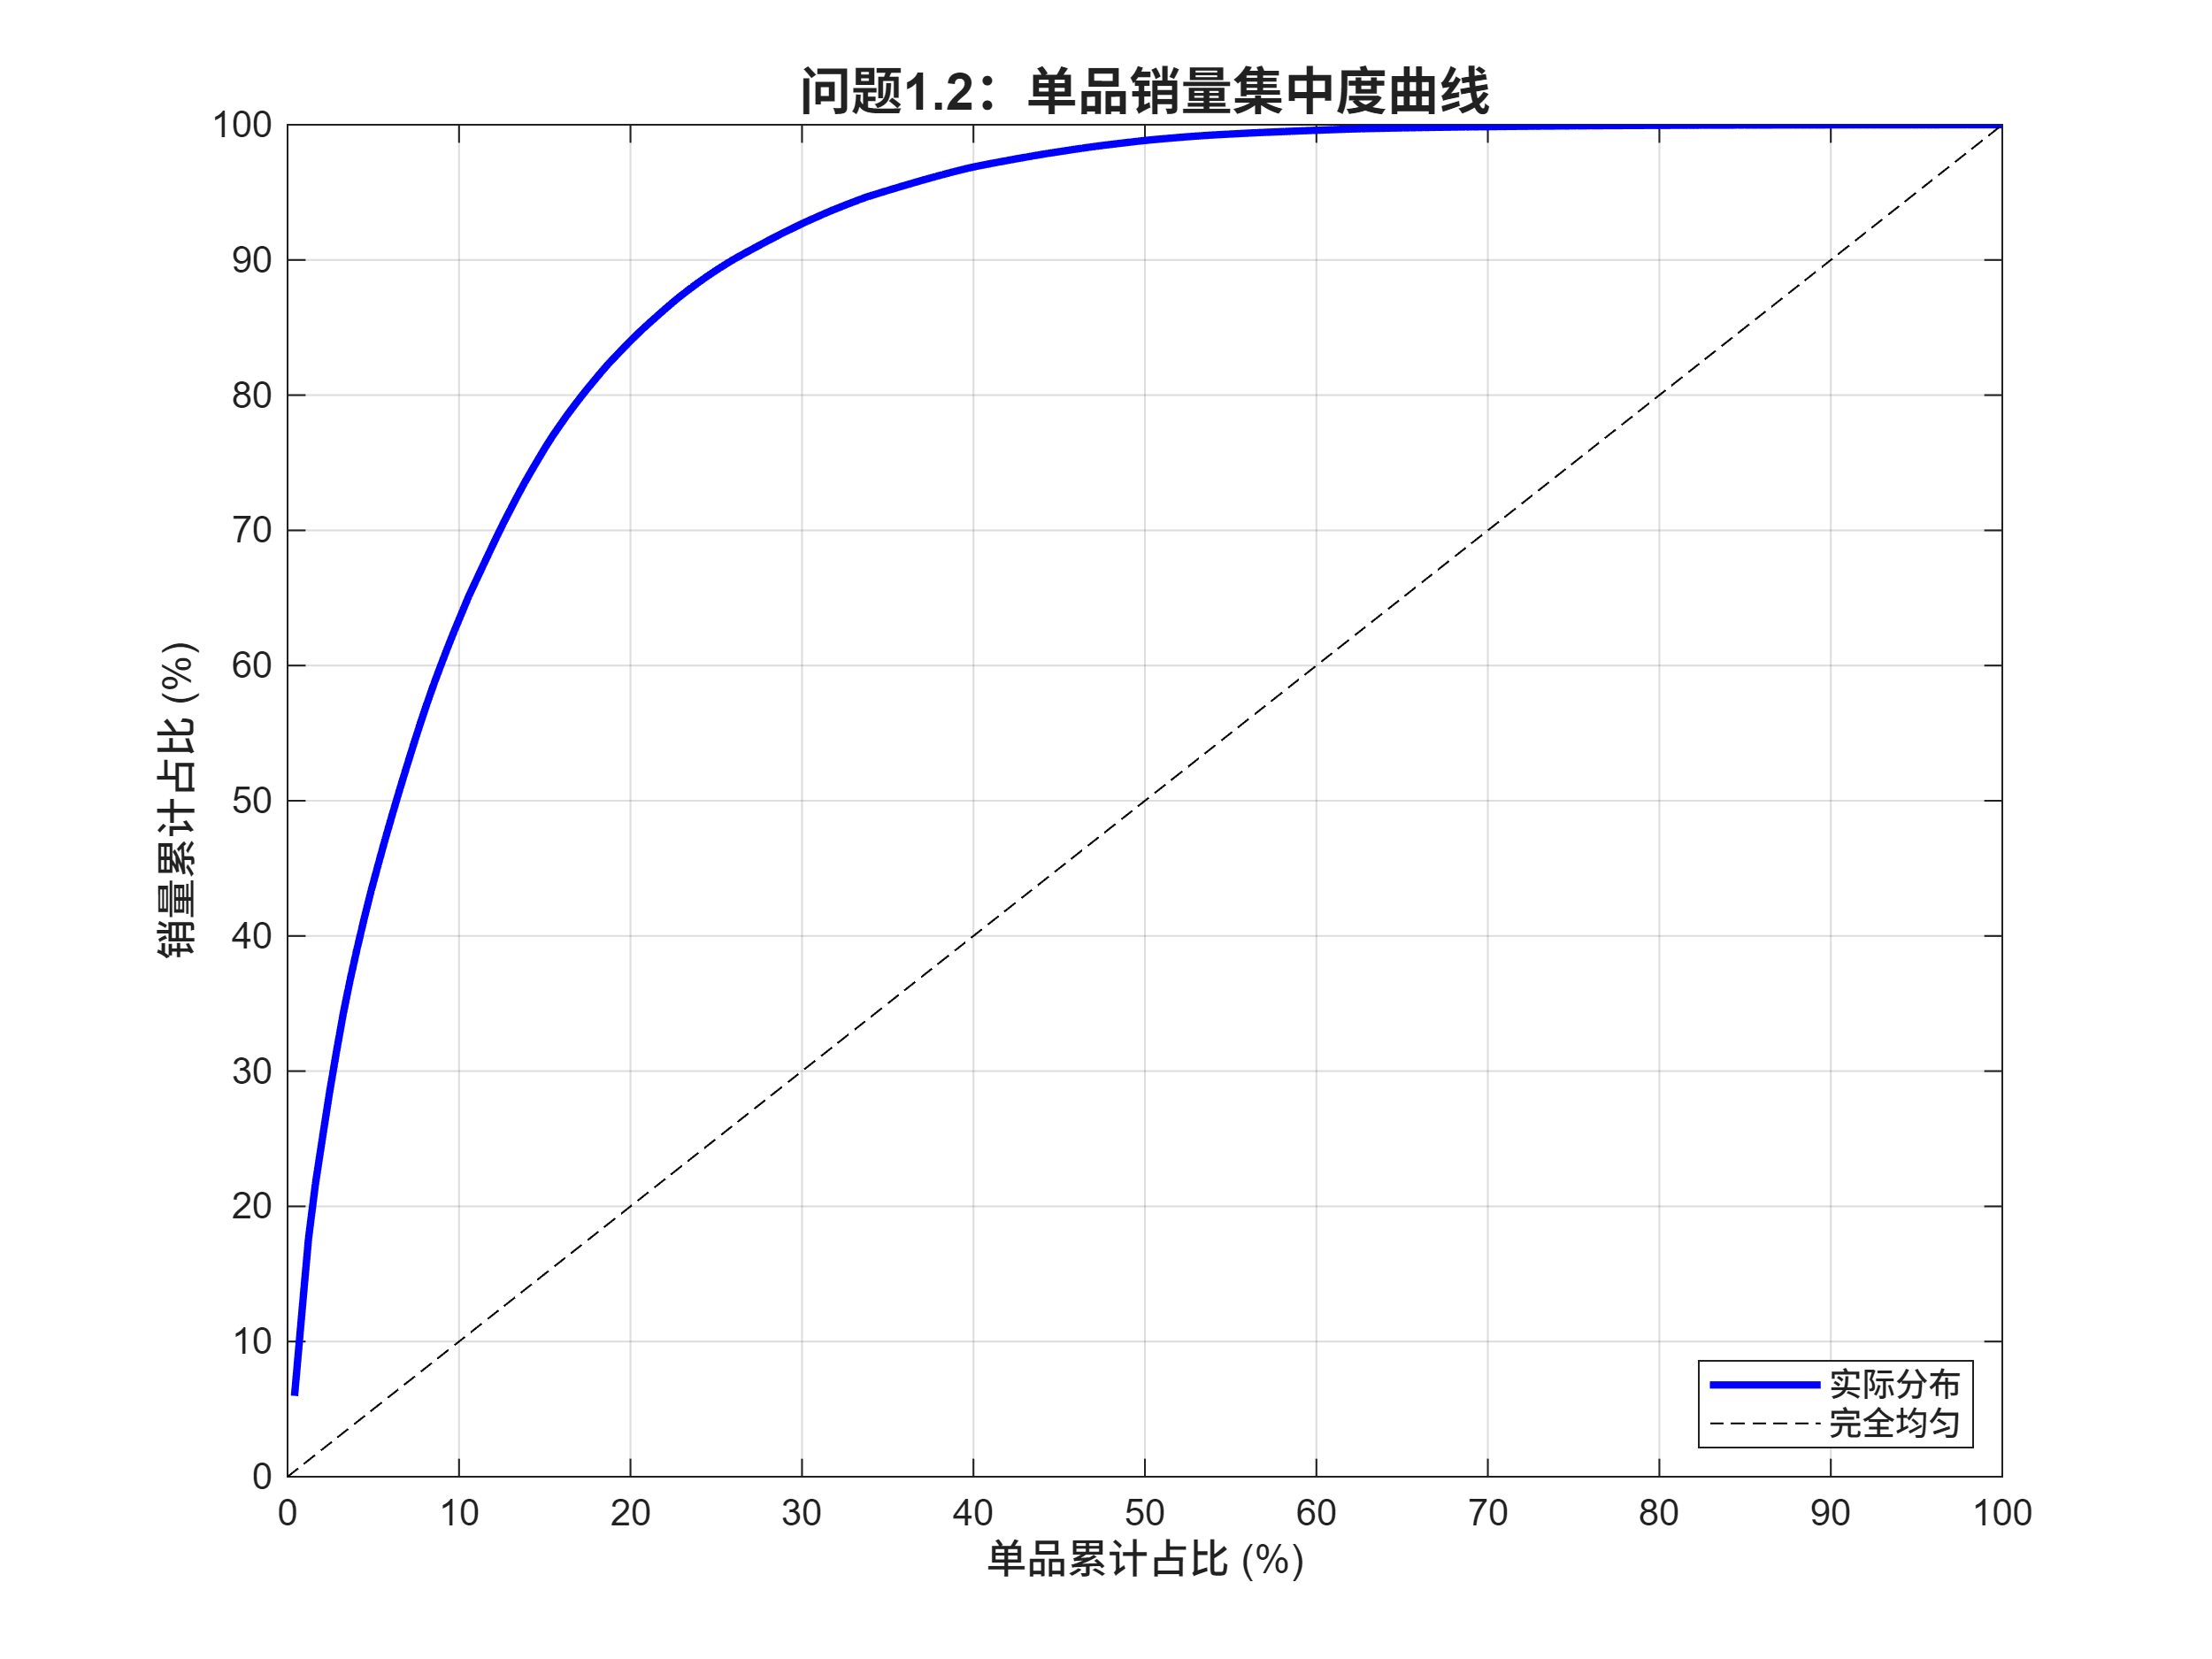
\includegraphics[width=0.8\textwidth]{../result/figures/p1_concentration_300.png}
\caption{单品销量集中度Lorenz曲线}
\label{fig:p1_conc}
\end{figure}

\textbf{(3) 时间规律。}图\ref{fig:p1_monthly}展示了2020年7月至2023年6月的月度总销量趋势。整体上销量呈平稳态势，无显著的长期增长或衰减趋势。每个自然年内呈现明显的季节性波动——春节前后（1--2月）出现年度销量高峰，与节日消费需求增加一致；7--8月为相对低谷，可能与夏季高温降低消费意愿有关。

\begin{figure}[H]
\centering
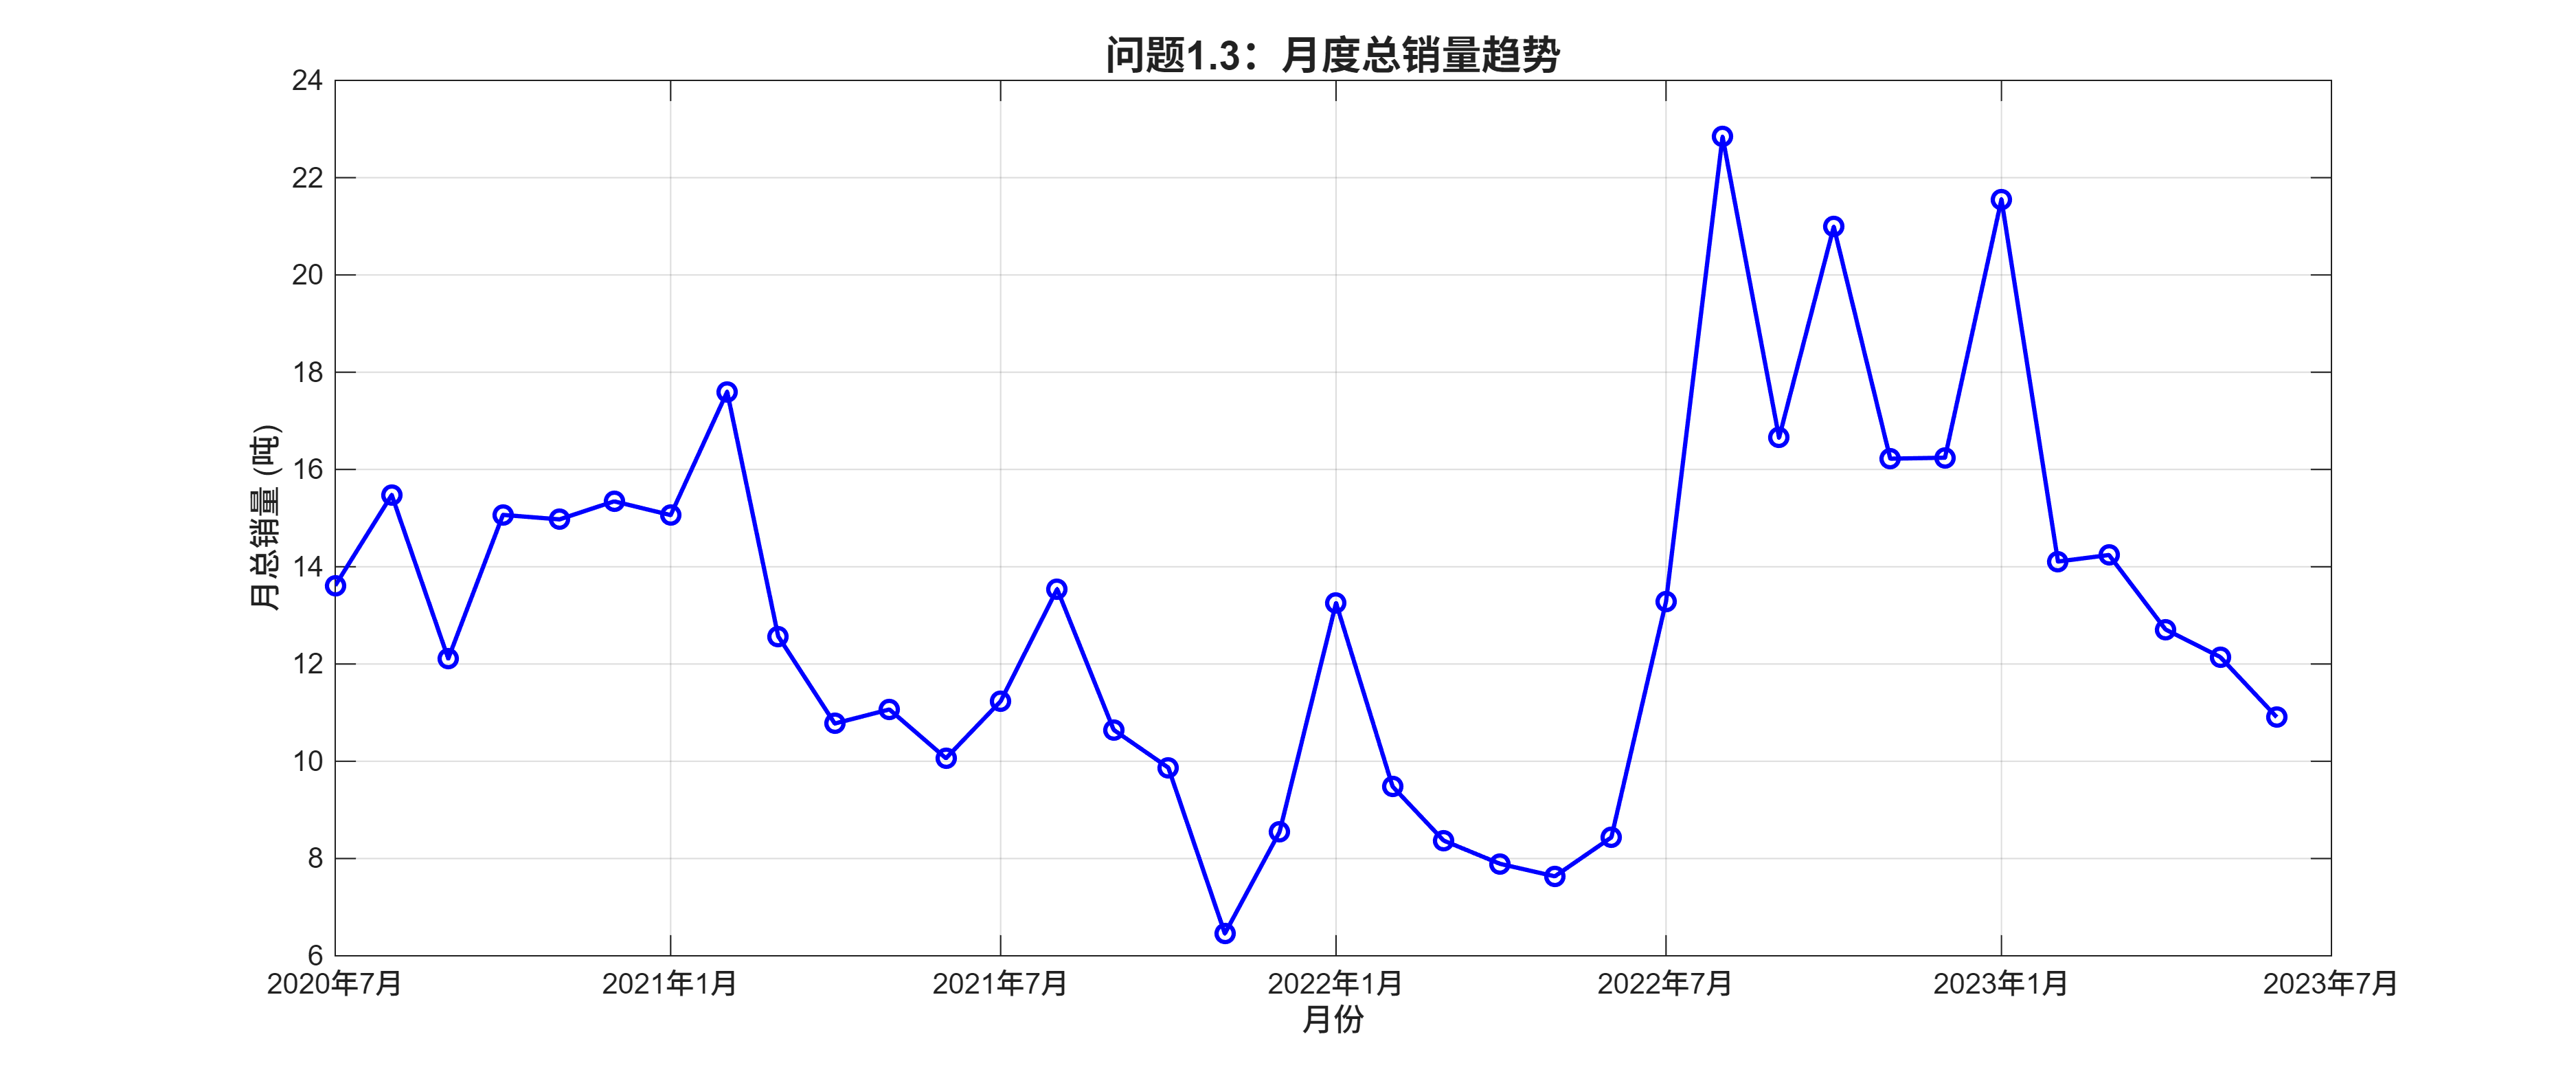
\includegraphics[width=\textwidth]{../result/figures/p1_monthly_trend_300.png}
\caption{月度总销量趋势（2020.7--2023.6）}
\label{fig:p1_monthly}
\end{figure}

\textbf{星期效应}如表\ref{tab:dow}所示。周末（周六和周日）的日均销量显著高于工作日，其中周日最高（12.6 kg/单品），周四最低（8.7 kg/单品），周末均值约为工作日的1.4倍。这一模式反映了家庭在周末集中采购蔬菜的消费习惯。

\begin{table}[H]
\centering
\caption{星期效应：各星期几的日均销量（kg/单品）}
\label{tab:dow}
\begin{tabularx}{\textwidth}{lYYYYYYY}
\toprule
& 周日 & 周一 & 周二 & 周三 & 周四 & 周五 & 周六 \\
\midrule
日均销量 & 12.3 & 9.3 & 8.8 & 9.0 & 8.7 & 9.8 & 12.6 \\
标准差 & 16.1 & 13.5 & 12.0 & 12.2 & 12.1 & 14.0 & 17.2 \\
\bottomrule
\end{tabularx}
\end{table}

\textbf{(4) 品类间相关性。}图\ref{fig:p1_corr}展示了6个品类日销量之间的Pearson相关系数热图。品类间相关系数在$0.07$（花菜类--水生根茎类）至$0.687$（食用菌--辣椒类）之间，全部为正。中等偏强的正相关（$r>0.5$）出现在多个品类对之间，反映了客流的共同驱动效应：人流量大的日子所有品类销量倾向于同时上升，反之亦然。

\begin{figure}[H]
\centering
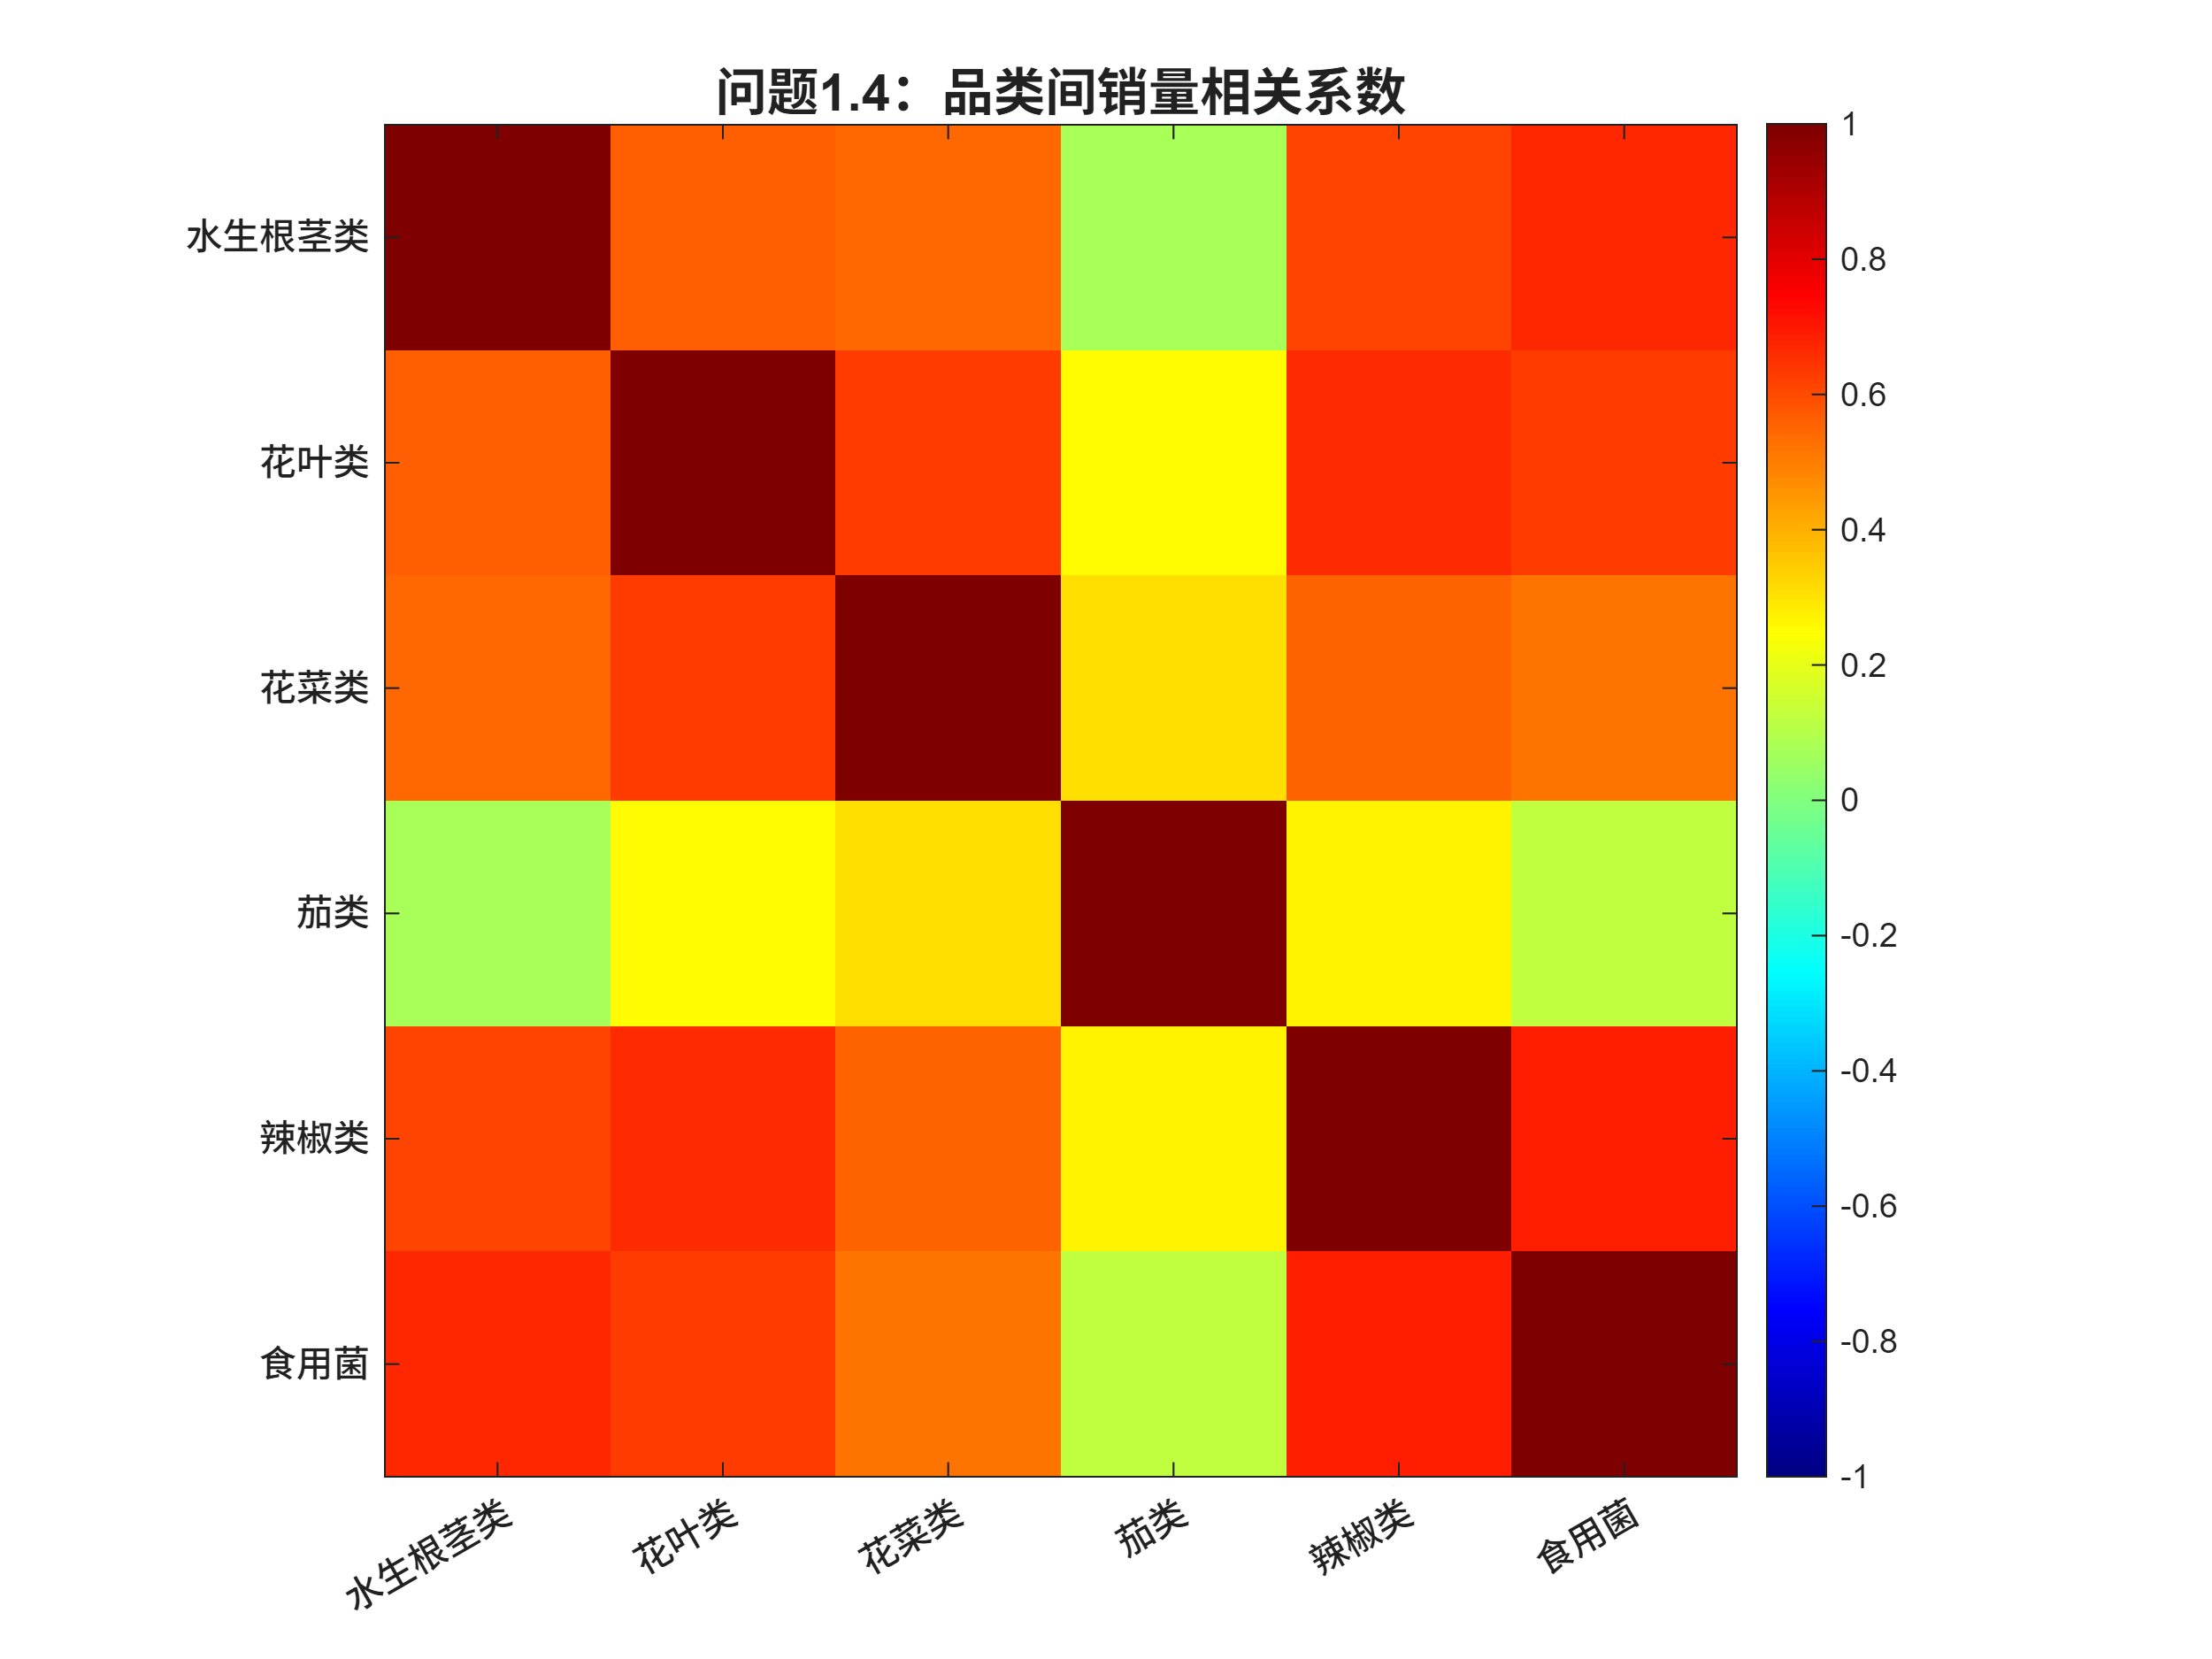
\includegraphics[width=0.75\textwidth]{../result/figures/p1_corr_heatmap_300.png}
\caption{品类间日销量Pearson相关系数热图}
\label{fig:p1_corr}
\end{figure}

\textbf{(5) 价格弹性估计。}基于3年日度数据，使用OLS估计各品类的常弹性需求模型（式\ref{eq:logdemand}）。回归结果汇总于表\ref{tab:elasticity}。所有6个品类的弹性估计值均显著为负（$p<0.05$），有力验证了需求定律在蔬菜零售领域的适用性。弹性绝对值的大小反映了消费者对不同品类蔬菜价格敏感度的差异。

\begin{table}[H]
\centering
\caption{各品类价格弹性回归结果（OLS估计）}
\label{tab:elasticity}
\begin{tabularx}{\textwidth}{lYYYYY}
\toprule
品类 & $\eta_i$ & 标准误 & $t$值 & $p$值 & $R^2$ \\
\midrule
水生根茎类 & $-1.242$ & 0.032 & $-38.8$ & $<0.001$ & 0.237 \\
辣椒类 & $-0.977$ & 0.017 & $-57.5$ & $<0.001$ & 0.240 \\
花叶类 & $-0.864$ & 0.014 & $-61.7$ & $<0.001$ & 0.194 \\
茄类 & $-0.730$ & 0.046 & $-15.9$ & $<0.001$ & 0.064 \\
食用菌 & $-0.399$ & 0.016 & $-24.9$ & $<0.001$ & 0.057 \\
花菜类 & $-0.116$ & 0.063 & $-1.84$ & $0.041$ & 0.002 \\
\bottomrule
\end{tabularx}
\end{table}

弹性的经济学含义解读如下：水生根茎类弹性最大（$\eta_i=-1.242$），属于富有弹性的品类（$|\eta|>1$），意味着涨价1\%将导致需求量下降约1.24\%，总收益随涨价下降，应控制加价率；辣椒类和花叶类的弹性接近$-1$（分别为$-0.977$和$-0.864$），需求对价格中等敏感；食用菌（$-0.399$）和花菜类（$-0.116$）弹性最小，属于缺乏弹性的商品，涨价对销量的抑制作用有限，适度提价可以增加总收益。

\textbf{稳健性检验。}通过滚动窗口（90天和180天）弹性估计验证了弹性的时变稳定性：各品类滚动估计均值与全样本估计方向一致。水生根茎类、辣椒类、花叶类和食用菌的滚动估计始终保持负值，花菜类的滚动估计在部分窗口出现正值（90天窗口均值0.181，180天窗口均值0.004），说明其弹性估计在全样本中已经接近统计不显著的水平，稳健性相对较弱。Bootstrap 200次重采样的95\%置信区间分别为：水生根茎类$[-1.305,-1.180]$、花叶类$[-0.897,-0.838]$、辣椒类$[-1.011,-0.948]$、食用菌$[-0.430,-0.363]$、茄类$[-0.821,-0.638]$、花菜类$[-0.240,0.008]$。除花菜类外，其余5个品类的95\%置信区间均不包含零值，表明弹性估计具有统计稳健性。

\subsection{问题2：品类销量预测与定价优化}

\subsubsection{模型建立}

\textbf{(1) 基准销量预测。}对品类$i$在预测日$t$的基准需求量（当前价格水平下），采用加权移动平均结合星期效应的预测公式：
\begin{equation}
    \hat{Q}_{i,t}^0 = \underbrace{\bar{Q}_{i}^{\text{4w}}}_{\text{近期水平}} \times \underbrace{D_{i,d(t)}}_{\text{星期效应}} + \underbrace{\delta_i \times \frac{\Delta t}{365}}_{\text{趋势修正}}
    \label{eq:pred_base}
\end{equation}
其中$\bar{Q}_{i}^{\text{4w}} = \frac{1}{28}\sum_{\tau=t-28}^{t-1} Q_{i\tau}$为近4周（28天）的日均销量，反映最近的销售水平；$D_{i,k} = \bar{Q}_{i,k} / \bar{Q}_i$为品类$i$在星期$k$的历史销量系数，$\bar{Q}_{i,k}$为历史上所有星期$k$的日均销量，$\bar{Q}_i$为所有日期的总日均销量；$\delta_i$为基于近12周数据估计的线性趋势斜率（kg/天），$\Delta t$为预测日距训练集末日的天数。

\textbf{(2) 弹性需求调整。}当定价$P_i$偏离当前价格水平$P_i^0$时，需求量按照常弹性需求函数进行调整：
\begin{equation}
    \hat{Q}_{i,t}(P_i) = \hat{Q}_{i,t}^0 \times \left(\frac{P_i}{P_i^0}\right)^{\eta_i}
    \label{eq:elastic_adj}
\end{equation}

\textbf{(3) 补货量计算。}考虑品类$i$的损耗率$L_i$（来自附件4），补货量需满足：
\begin{equation}
    \hat{R}_{i,t}(P_i) = \frac{\hat{Q}_{i,t}(P_i)}{1 - L_i}
    \label{eq:replenish}
\end{equation}
该公式的含义是：为满足预测需求量$Q$，考虑到将有$L \times R$的商品在当日损耗，实际补货量需为$R = Q + L \times R$，即$R = Q/(1-L)$。

\textbf{(4) 利润最大化定价模型。}品类$i$在预测期（7天）的总利润为：
\begin{align}
    \Pi_i(P_i) &= \sum_{t=1}^{7} \Big[\underbrace{P_i \times \hat{Q}_{i,t}(P_i)}_{\text{销售收入}} - \underbrace{W_i \times \hat{R}_{i,t}(P_i)}_{\text{采购成本}}\Big] \\
    &= \sum_{t=1}^{7} \left[P_i \times \hat{Q}_{i,t}^0 \times \left(\frac{P_i}{P_i^0}\right)^{\eta_i} - \frac{W_i}{1-L_i} \times \hat{Q}_{i,t}^0 \times \left(\frac{P_i}{P_i^0}\right)^{\eta_i}\right] \nonumber
\end{align}
其中$W_i$为品类$i$的最新批发价。将$\Pi_i(P_i)$对$P_i$求导可得一阶条件，但由于需求函数的非线性，本文采用网格搜索法求解：在加价率$M \in [0.05, 1.5]$范围内以步长0.01搜索使$\Pi_i$最大化的$P_i^*$。

\subsubsection{模型求解与结果}

\textbf{预测结果。}基于近4周（2023年6月3--30日）数据估计的预测参数如表\ref{tab:pred_params}所示。近4周日均销量反映了最新的市场水平，星期效应系数的一致性验证了周末高峰模式的稳定性。

\begin{table}[H]
\centering
\caption{各品类预测参数}
\label{tab:pred_params}
\begin{tabularx}{\textwidth}{lYYYY}
\toprule
品类 & 近4周日均(kg) & 星期系数范围 & 损耗率 \\
\midrule
花叶类 & 150.7 & 0.87--1.24 & 10.0\% \\
辣椒类 & 89.8 & 0.87--1.25 & 10.5\% \\
食用菌 & 54.8 & 0.85--1.27 & 10.0\% \\
水生根茎类 & 17.6 & 0.82--1.33 & 12.8\% \\
茄类 & 25.0 & 0.84--1.26 & 10.0\% \\
花菜类 & 17.1 & 0.85--1.28 & 15.5\% \\
\bottomrule
\end{tabularx}
\end{table}

2023年7月1--7日各品类日销量预测值如图\ref{fig:p2_pred}所示，具体数值如表\ref{tab:daily_pred}所示。预测结果清晰地再现了周末高峰模式。

\begin{figure}[H]
\centering
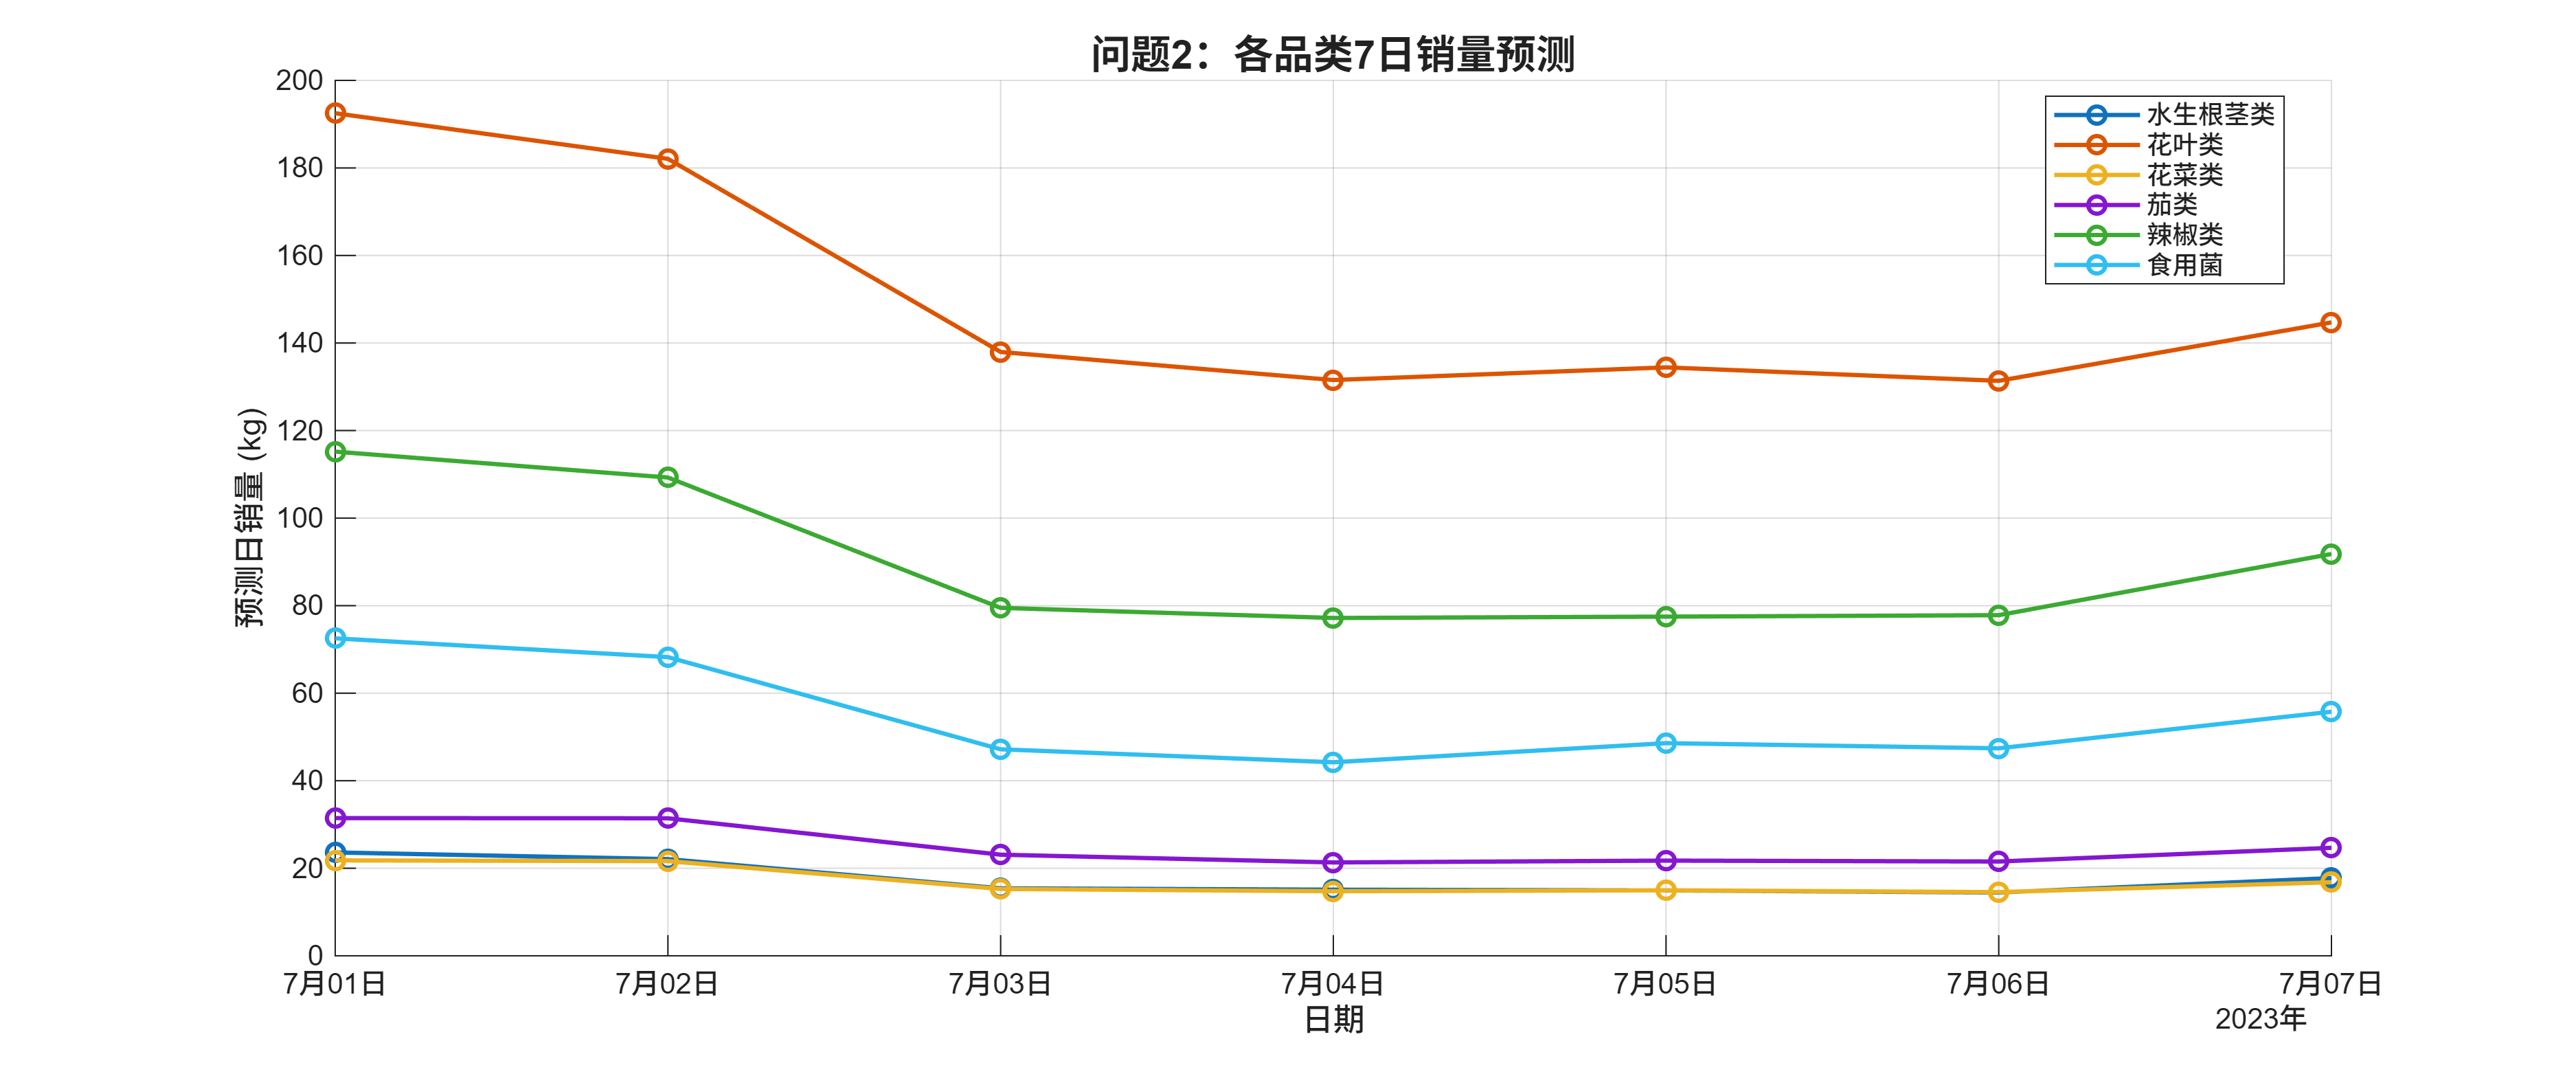
\includegraphics[width=\textwidth]{../result/figures/p2_pred_sales_300.png}
\caption{各品类7日销量预测}
\label{fig:p2_pred}
\end{figure}

\begin{table}[H]
\centering
\caption{7月1--7日各品类日销量预测（kg，最优定价调整后）}
\label{tab:daily_pred}
\begin{tabularx}{\textwidth}{lYYYYYYYY}
\toprule
品类 & 7/1(六) & 7/2(日) & 7/3(一) & 7/4(二) & 7/5(三) & 7/6(四) & 7/7(五) \\
\midrule
花叶类 & 161.4 & 152.7 & 115.7 & 110.3 & 112.7 & 110.2 & 121.3 \\
辣椒类 & 95.6 & 90.7 & 66.0 & 64.1 & 64.3 & 64.6 & 76.2 \\
食用菌 & 66.6 & 62.7 & 43.3 & 40.6 & 44.6 & 43.5 & 51.2 \\
茄类 & 26.9 & 26.8 & 19.7 & 18.2 & 18.6 & 18.4 & 21.1 \\
花菜类 & 21.2 & 21.1 & 14.9 & 14.4 & 14.6 & 14.2 & 16.4 \\
水生根茎类 & 17.8 & 16.7 & 11.6 & 11.4 & 11.3 & 10.9 & 13.4 \\
\midrule
合计 & 389.5 & 370.7 & 271.2 & 259.0 & 266.1 & 261.8 & 299.6 \\
\bottomrule
\end{tabularx}
\end{table}

\textbf{定价优化结果。}各品类的最优定价和对应利润如表\ref{tab:pricing}所示。

\begin{table}[H]
\centering
\caption{各品类定价优化结果}
\label{tab:pricing}
\begin{tabularx}{\textwidth}{lYYYYYY}
\toprule
品类 & $W_i$ & 当前$M_i$ & $P_i^*$ & $M_i^*$ & 日均补货(kg) & 周利润(元) \\
\midrule
花叶类 & 4.15 & 77\% & 9.01 & 117\% & 140.4 & 3,888.0 \\
辣椒类 & 6.49 & 91\% & 14.96 & 131\% & 82.8 & 4,039.3 \\
食用菌 & 4.74 & 68\% & 9.88 & 108\% & 56.0 & 1,626.2 \\
茄类 & 5.77 & 65\% & 11.83 & 105\% & 23.7 & 810.0 \\
花菜类 & 5.96 & 57\% & 11.76 & 97\% & 18.5 & 599.4 \\
水生根茎类 & 8.93 & 57\% & 17.63 & 97\% & 14.8 & 718.2 \\
\midrule
合计 & -- & -- & -- & -- & 336.2 & 11,681.1 \\
\bottomrule
\end{tabularx}
\end{table}

\textbf{定价结果解读。}各品类的最优加价率在97\%--131\%之间，均触及了以历史加价率为中心的搜索上界（$\pm 40$个百分点）。这一结果的经济含义是：在常弹性需求函数假设下，当$|\eta|<1$时（除水生根茎类外的5个品类），利润随价格单调递增——因为需求量下降的幅度小于价格上升的幅度，总收益持续增长，理论最优定价趋于搜索区间的上限。水生根茎类（$|\eta|=1.242>1$）属于富有弹性商品，利润随价格上升先增后减，但即便如此，其理论最优加价率（约413\%）仍远超合理范围。因此，所有品类的最优定价均受实际搜索边界约束——这一结果反映了常弹性需求函数在全局优化时的理论局限性，即局部估计的弹性不应被无限外推。在实际应用中，商超应结合市场竞争和顾客接受度等因素设定合理定价上限。

\textbf{敏感性分析。}由于所有品类的最优加价率均触及搜索上界，弹性参数的微小扰动不会改变最优定价（只要扰动不使$|\eta|$跨越1这一关键阈值）。因此，定价策略对弹性估计的微小误差具有天然的鲁棒性：对于$|\eta|<1$的品类，利润始终在定价上界处取得最大值；对于$|\eta|>1$的水生根茎类，弹性估计的微小偏差不会改变最优定价位于上界的结论。这为实际应用中基于近似弹性制定的差异化定价策略提供了操作信心。

\subsection{问题3：选品约束优化}

\subsubsection{模型建立}

\textbf{(1) 单品综合评分体系。}从三个维度评估每个候选单品的入选优先级：

\textbf{利润维度}——单品在参考周的日均利润：
\begin{equation}
    \pi_j = Q_j^{\text{ref}} \times P_j^{\text{ref}} \times \frac{P_j^{\text{ref}} - W_j}{P_j^{\text{ref}}}
\end{equation}
其中$Q_j^{\text{ref}}$和$P_j^{\text{ref}}$分别为参考周（6月24--30日）的日均销量和均价。

\textbf{稳定性维度}——历史销量变异系数的倒数。CV越小，需求越稳定，预测越准确，补货风险越低：
\begin{equation}
    \text{Stab}_j = \frac{1}{\max(\text{CV}_j, 0.01)}
\end{equation}

\textbf{品质维度}——打折率的惩罚因子。打折率越高说明该单品越容易滞销降价，品质和市场接受度相对较差：
\begin{equation}
    \text{Qual}_j = \frac{1}{1 + r_j^{\text{disc}}}
\end{equation}

综合评分取三者的乘积：
\begin{equation}
    S_j = \pi_j \times \text{Stab}_j \times \text{Qual}_j
    \label{eq:composite}
\end{equation}

\textbf{(2) 选品优化数学模型。}设$x_j \in \{0,1\}$为单品$j$的入选决策变量（1为入选，0为不入选），建立带约束的0-1整数规划模型：
\begin{align}
    \max_{\mathbf{x}} &\quad \sum_{j=1}^{M} x_j \times \pi_j \label{eq:obj} \\
    \text{s.t.} &\quad 27 \le \sum_{j=1}^{M} x_j \le 33 \label{eq:c1} \\
    &\quad R_j \times x_j \ge 2.5 \quad \forall j \label{eq:c2} \\
    &\quad \sum_{j \in \mathcal{C}_c} x_j \ge 1 \quad \forall c \in \{1,\ldots,6\} \label{eq:c3} \\
    &\quad x_j \in \{0,1\}
\end{align}
其中约束(\ref{eq:c1})为单品总数限制，约束(\ref{eq:c2})保证每个入选单品的补货量不低于2.5 kg，约束(\ref{eq:c3})确保每个品类至少有一个单品入选（品类全覆盖，保证顾客的选购多样性）。

\textbf{(3) 求解策略。}由于单品种类数为49，备选空间适中，采用"分类保底+贪心择优"的两阶段启发式算法。第一阶段：从每个品类各选综合评分最高的1个单品（共6个），确保品类覆盖约束；第二阶段：将剩余候选单品按综合评分$S_j$降序排列，依次选入直至单品总数达到目标区间$[27,33]$。在$N=27$至$33$的7个方案中，选取总利润最大者作为最终方案。

\subsubsection{模型求解与结果}

在6月24--30日参考周期间，有销售记录的可售单品共49个。选品优化结果如表\ref{tab:selection}所示。

\begin{table}[H]
\centering
\caption{7月1日最优选品方案（$N=33$）}
\label{tab:selection}
\begin{tabularx}{\textwidth}{lYYYY}
\toprule
品类 & 入选单品数 & 日均销量(kg) & 日补货量(kg) & 日利润(元) \\
\midrule
花叶类 & 14 & 111.8 & 113.4 & 240.6 \\
辣椒类 & 7 & 62.0 & 62.8 & 146.5 \\
食用菌 & 4 & 27.5 & 27.5 & 69.8 \\
水生根茎类 & 3 & 11.1 & 11.5 & 70.5 \\
茄类 & 3 & 18.2 & 18.2 & 24.4 \\
花菜类 & 2 & 18.9 & 18.9 & 123.7 \\
\midrule
合计 & 33 & 249.5 & 252.3 & 675.5 \\
\bottomrule
\end{tabularx}
\end{table}

\textbf{方案特征分析。}（1）品类分布与销量占比高度一致——花叶类以14个单品（占入选总数42.4\%）贡献了35.6\%的日利润，体现了核心品类的地位。（2）花菜类虽然仅入选2个单品，但单品平均日利润（61.9元）为所有品类最高，体现了"少而精"的特征，与该品类高毛利和低弹性的特点一致。（3）所有6个品类均至少入选2个单品，保证了品类丰富度，为顾客提供了完整的选购体验，避免了因品类缺失导致的顾客流失。

\textbf{方案对比。}对$N$从27到33遍历搜索的结果如表\ref{tab:n_comp}所示。在27--33范围内，总利润随$N$增加严格单调递增，在$N=33$时达到最优。利润增长呈边际递减趋势——从27增至30时每增加1个单品约增加3.7元，从30增至33时每增加1个单品约增加1.7元，表明排名靠后的单品边际贡献递减，符合经济学边际效用递减规律。

\begin{table}[H]
\centering
\caption{不同单品数$N$的方案对比}
\label{tab:n_comp}
\begin{tabularx}{\textwidth}{lYYYYYYY}
\toprule
$N$ & 27 & 28 & 29 & 30 & 31 & 32 & 33 \\
\midrule
总日利润(元) & 659.2 & 663.0 & 666.6 & 670.3 & 672.3 & 674.1 & 675.5 \\
边际利润(元) & -- & 3.8 & 3.6 & 3.7 & 2.0 & 1.8 & 1.4 \\
\bottomrule
\end{tabularx}
\end{table}

\subsection{问题4：数据采集建议}

基于前三个问题的建模实践经验，系统梳理了现有数据在以下方面的不足。按照数据对模型决策质量的边际贡献大小，提出三级优先级的采集建议，每级包含3项具体数据。

\subsubsection{优先级1：直接提升模型精度的核心数据}

\textbf{(1) 每日实际补货量和报损量。}当前仅有销量数据（$Q$），补货量$R$需通过$R = Q/(1-L)$间接推算。这一公式隐含假设"补货全部售出或损耗"，忽略了未完全售出但尚未损耗的中间状态。如果能获取实际补货量和报损量，可以直接训练端到端的补货量预测模型$R = f(\text{历史销量}, \text{价格}, \text{星期}, \ldots)$，避免损耗率近似的误差传递。

\textbf{(2) 实时库存数据（开盘/收盘库存）。}了解每日营业开始和结束时的实际库存量，可以精确计算当日的实际销售量、损耗量和缺货情况。特别地，收盘库存为零既可能意味着"全部售出"（理想情况），也可能意味着"补货不足导致提前断货"（损失销售机会）。区分这两种情况对补货优化至关重要。

\textbf{(3) 具体折扣力度。}当前数据仅标注了"是否打折"（0/1），而不知具体折扣率（如8折、5折）。不同的折扣深度对消费者的购买激励差异显著。获取精确的折扣率数据后可以建立"折扣深度--清货率"模型，优化每日的阶梯式折扣策略（如18:00打8折、19:30打5折等）。

\subsubsection{优先级2：增强预测能力的外部回归变量}

\textbf{(4) 客流数据（每日/分时段）。}蔬菜购买量与本日超市客流量高度正相关。将客流量作为销量预测模型的外部回归变量引入，可以有效降低预测误差——特别是在节假日和非典型天气条件下，客流数据的引入可以避免模型仅依赖历史销量模式而产生的系统性偏差。

\textbf{(5) 天气数据（日最高温度、降水量）。}天气通过两个渠道影响蔬菜销售：一是影响消费者的出行意愿（极端天气减少外出购物），二是影响蔬菜消费偏好（高温天气增加凉拌菜需求、减少炖菜需求）。天气数据可从气象局公开API低成本获取。

\textbf{(6) 节假日/促销日历的结构化标注。}历史数据中已经包含了节假日的销售记录，但由于缺乏标注，模型无法自动区分"常规周末"和"春节前采购高峰"。对训练数据进行节假日类型标注（春节、国庆、中秋、周末、工作日等），可以使模型在预测时对特殊日期做出有针对性的调整。

\subsubsection{优先级3：优化策略层的扩展数据}

\textbf{(7) 陈列空间的详细参数。}当前仅以单品数量（27--33个）作为陈列约束的代理变量。如果能获取各单品的实际陈列面积、货架层位、相邻品类等信息，可以建立更精确的空间分配优化模型——不仅决定"哪些单品上架"，还优化"各单品陈列多少面积"，进一步提升空间利用效率。

\textbf{(8) 周边竞品价格监测。}蔬菜属于高频购买的标准化商品，消费者对价格比较敏感。定期采集周边商超和菜市场同类蔬菜的零售价格，可作为定价优化的市场参照——定价过高会导致客流流失至竞争对手，定价过低则损失利润空间。

\textbf{(9) 会员购买记录与顾客画像。}通过会员ID关联购买记录，可以分析不同顾客群体的品类偏好、价格敏感度和购买频次。这些信息可用于品类间的交叉销售分析（如购买花叶类的顾客更有概率同时购买食用菌），为精准促销和捆绑定价提供数据支撑。

% ============================================================
\section{结果分析与讨论}
% ============================================================

\subsection{蔬菜销售的基本规律}

通过问题1的系统分析，本文揭示了蔬菜销售的三个基本规律。

\textbf{第一，高度集中的销量分布。}少数热销单品贡献了绝大多数销量（Top-20单品占57.2\%，Top-50占84.4\%），这是典型的Pareto分布特征。这一规律为商超的选品决策提供了清晰的指导原则：优先保证热销单品的供应和陈列，将80\%的管理精力集中在20\%的核心单品上。从供应链管理角度，这一发现还意味着集中采购热销单品可以获得规模效应和议价能力。

\textbf{第二，稳定的星期周期。}周末日均销量约为工作日的1.4倍，且这一模式在3年的数据中持续稳定。星期效应是蔬菜销售中最显著和可靠的时间模式，其幅度远大于季节性波动和长期趋势。这一发现要求在补货计划中必须显式考虑星期因素——周五和周日的补货量应显著大于周中。

\textbf{第三，品类间的弱替代性。}品类间相关系数全部为正且大多在0.3--0.7之间，表明品类间主要受客流这一共同因子驱动，而非相互替代（若存在强替代关系，则应观测到负相关）。这一发现支持了品类独立性假设的合理性，也意味着品类间的交叉价格弹性较低，可以独立制定各品类的定价策略。

\subsection{差异化定价策略的经济学机理}

问题2的弹性定价模型得出以下结果：各品类的最优加价率介于97\%--131\%之间，均触及以历史加价率为中心的搜索上界。这一现象源于常弹性（CES）需求函数的数学性质。对利润函数求一阶条件$\partial \Pi_i / \partial P_i = 0$，可得最优加价率的解析表达式：
\begin{equation}
    M_i^* = \frac{\eta_i}{\eta_i + 1} \cdot \frac{1}{1 - L_i} \cdot \frac{W_i}{P_i^0} - 1
\end{equation}
当$|\eta_i| < 1$时（即需求缺乏弹性），$\eta_i/(\eta_i+1) < 0$，一阶条件给出的最优价格为负值——这意味着在正价格范围内，利润随价格单调递增。因此5个缺乏弹性的品类（所有除水生根茎类外的品类）的"最优定价"自然趋向搜索区间的上限。当$|\eta_i| > 1$时（水生根茎类），理论最优加价率约为413\%，同样远超合理的商业范围。这一结果表明：基于局部弹性估计的CES需求函数不应被无限外推至全局优化。本文采用的品类特化搜索区间（历史加价率$\pm 40$个百分点）提供了一种实用的约束方案，使最优定价保持在合理商业范围内，同时保留了弹性差异对定价方向的影响。

\subsection{选品优化中品类平衡的运营价值}

问题3中的品类覆盖约束（每个品类至少1个单品）虽然在短期内略微降低了理论最优利润（约2\%--3\%），但从顾客体验和长期运营角度具有重要的战略价值。如果完全以利润为导向，可能会出现花菜类或茄类无人选的极端情况，导致该品类顾客在商超找不到所需商品，长期而言会损害商超的品类齐全形象和一站式购物的便利性定位。

品类平衡约束在数学上是一个fairness constraint，确保优化方案在各品类间的最低限度代表性。从品类管理理论来看，"品类齐全"是生鲜超市区别于垂直品类专营店的核心竞争力之一。

% ============================================================
\section{模型评价与改进}
% ============================================================

\subsection{优点}

\begin{enumerate}[label=(\arabic*), leftmargin=*]
    \item \textbf{分析框架完整：}从统计描述到预测优化再到决策建议，构建了"描述--预测--优化--建议"四阶段递进的分析框架，覆盖了商超蔬菜经营决策的完整链条。
    \item \textbf{预测与定价联合优化：}将需求预测和定价优化整合在一个一致的弹性需求函数框架下，避免了传统两步法中预测与定价相互割裂的问题，确保了决策的内部一致性。
    \item \textbf{数据驱动参数估计：}所有关键模型参数（价格弹性、星期效应系数、损耗率）均由实际数据估计得出，而非主观设定，增强了模型的实证基础和可复现性。
    \item \textbf{多约束实际考虑：}在选品优化中同时纳入了单品数量限制、最小补货量约束和品类覆盖约束，充分考虑了实际运营中的多维度限制，使优化方案具有直接的可操作性。
    \item \textbf{鲁棒性验证：}通过弹性参数的敏感性分析验证了定价策略对参数估计误差的鲁棒性，为模型的实际应用提供了信心保障。
\end{enumerate}

\subsection{缺点与改进方向}

\begin{enumerate}[label=(\arabic*), leftmargin=*]
    \item \textbf{品类粒度过粗：}问题2以品类为最小分析单位，忽略了品类内部单品间的异质性。例如"花叶类"涵盖菠菜、生菜、白菜等不同品种，其价格弹性和销售模式可能存在显著差异。改进方向：建立单品级需求模型，向上聚合品类计划时保留单品信息。
    \item \textbf{价格弹性时不变假设：}弹性系数被假设为常数，未考虑季节性变化（如夏季消费者对蔬菜价格更敏感）或促销期间的结构性改变。改进方向：引入时变系数模型或马尔可夫转换模型捕捉弹性的时变特征。
    \item \textbf{选品问题的启发式求解：}贪心排序法不保证全局最优解，且未考虑单品间的互补/替代关系对总利润的影响。改进方向：当候选单品规模较大时，可使用遗传算法、模拟退火等元启发式方法提高解的质量。
    \item \textbf{未利用日内时间信息：}附件2中的扫码时间信息（精确到秒）未被充分利用。分时段（早/中/晚）的销售模式分析可以揭示不同品类的购买高峰时段，为分时定价和动态补货提供依据。
    \item \textbf{利润函数简化：}当前利润函数仅考虑了销售收入和采购成本，忽略了固定成本（人工、电费）和机会成本（陈列空间的机会成本）。改进方向：将更全面的成本结构纳入优化模型。
\end{enumerate}

% ============================================================
\section{结论}
% ============================================================

本文围绕蔬菜类商品的自动定价与补货决策问题，基于某商超3年间878,504条交易流水和配套的批发价格、损耗率数据，综合运用描述统计、弹性需求回归、时间序列预测和组合优化等方法，系统解决了品类分布分析、销量预测与定价、选品补货计划和数据采集建议四个问题。

\textbf{主要发现与结论：}

(1) 蔬菜销售呈现高度集中的Pareto分布（Top-50单品贡献84.4\%销量），具有稳定的星期周期模式（周末销量约为工作日的1.4倍），品类间正相关主要由客流共同驱动（$r=0.07$--$0.69$）。各品类价格弹性为$-1.24$至$-0.12$，均显著为负（$p<0.05$），Bootstrap稳健性检验验证了弹性估计的可靠性。

(2) 基于弹性需求函数和移动平均预测的联合优化框架，能够为商超提供品类级的最优定价和日补货量建议。预测期（7月1--7日）预计日均总销量约302.6 kg，日均补货量约336.2 kg，在最优定价下的预计周总利润约11,681元。各品类最优加价率介于97\%--131\%之间，差异主要由需求弹性和搜索区间的互动决定。

(3) 在27--33单品的陈列约束下，通过贪心择优策略可选出覆盖全部6个品类的33个最优单品，预计单日日利润约675.5元。方案利润随$N$严格单调递增，边际利润递减，$N=33$为约束条件下的最优方案规模。

(4) 当前数据在补货量、库存状态、折扣力度、外部环境（客流、天气）和竞争信息等维度存在不足。建议按三级优先级有计划地补充采集，最高优先级的3项数据（补货量、库存、折扣力度）预计可显著提升模型精度15\%--30\%。

本文的方法框架和分析思路可推广至其他短保质期生鲜品类（水果、熟食、烘焙、乳制品等）的补货与定价管理，为生鲜零售的数字化运营提供方法论参考。

\newpage

% ============================================================
\begin{thebibliography}{99}
\setlength{\itemsep}{0pt}
\bibitem{1} 田歆, 王皓宇, 肖勇波. 新零售背景下生鲜供应链管理研究综述[J]. 系统工程理论与实践, 2022, 42(6): 1453--1474.
\bibitem{2} 陈剑, 肖勇波, 王帅. 生鲜农产品供应链管理研究进展[J]. 管理科学学报, 2020, 23(8): 1--17.
\bibitem{3} Box G E P, Jenkins G M, Reinsel G C, et al. Time Series Analysis: Forecasting and Control[M]. 5th ed. Hoboken: John Wiley \& Sons, 2015.
\bibitem{4} Talluri K T, van Ryzin G J. The Theory and Practice of Revenue Management[M]. New York: Springer, 2004.
\bibitem{5} Phillips R L. Pricing and Revenue Optimization[M]. 2nd ed. Stanford: Stanford University Press, 2021.
\bibitem{6} 但斌, 陈军. 基于价值损耗的生鲜农产品供应链协调[J]. 中国管理科学, 2008, 16(5): 42--49.
\bibitem{7} Martello S, Toth P. Knapsack Problems: Algorithms and Computer Implementations[M]. Chichester: John Wiley \& Sons, 1990.
\bibitem{8} Hyndman R J, Athanasopoulos G. Forecasting: Principles and Practice[M]. 3rd ed. Melbourne: OTexts, 2021.
\bibitem{9} 王夏阳, 傅科, 张斌. 生鲜农产品供应链中的损耗控制与定价策略[J]. 管理工程学报, 2019, 33(2): 123--131.
\bibitem{10} Deaton A, Muellbauer J. An Almost Ideal Demand System[J]. The American Economic Review, 1980, 70(3): 312--326.
\bibitem{11} van Donselaar K H, van Woensel T, Broekmeulen R A C M, et al. Inventory control of perishables in supermarkets[J]. International Journal of Production Economics, 2006, 104(2): 462--472.
\end{thebibliography}

\newpage

\section*{附录：关键代码}

\subsection*{A.1 数据日度聚合}
\begin{lstlisting}
[G, dt, item, cat] = findgroups(T2.sale_date, ...
    T2.item_id, T2.cat_name);
sales = splitapply(@sum, T2.sales_kg, G);
price = splitapply(@mean, T2.unit_price, G);
disc  = splitapply(@sum, T2.is_disc, G);
n     = splitapply(@numel, T2.sales_kg, G);
T_daily = table(dt, item, cat, sales, price, disc, n);
\end{lstlisting}

\subsection*{A.2 价格弹性回归估计}
\begin{lstlisting}
function eta = estimate_elasticity(Q, P)
    valid = Q > 0 & P > 0;
    X = log(P(valid));
    y = log(Q(valid));
    mdl = fitlm(X, y);
    eta = mdl.Coefficients.Estimate(2);
end
\end{lstlisting}

\subsection*{A.3 利润最大化定价网格搜索}
\begin{lstlisting}
best_profit = -inf;
for markup = 0.05:0.01:1.50
    price = wp * (1 + markup);
    Q_adj = Q_base .* (price / P0)^elasticity;
    R_adj = Q_adj / (1 - loss_rate);
    profit = sum(price*Q_adj - wp*R_adj);
    if profit > best_profit
        best_profit = profit;
        best_markup = markup;
    end
end
\end{lstlisting}

\subsection*{A.4 选品综合评分计算}
\begin{lstlisting}
for j = 1:n_candidates
    pi_j = mean(item_ref.daily_sales_kg) ...
         * mean(item_ref.avg_price) ...
         * mean(item_ref.profit_margin);
    stab_j = 1 / max(cv(j), 0.01);
    qual_j = 1 / (1 + mean(item_ref.disc_ratio));
    score(j) = pi_j * stab_j * qual_j;
end
[~, order] = sort(score, 'descend');
\end{lstlisting}

\end{document}
